% Options for packages loaded elsewhere
\PassOptionsToPackage{unicode}{hyperref}
\PassOptionsToPackage{hyphens}{url}
\PassOptionsToPackage{dvipsnames,svgnames,x11names}{xcolor}
%
\documentclass[
  letterpaper,
  DIV=11,
  numbers=noendperiod]{scrreprt}

\usepackage{amsmath,amssymb}
\usepackage{iftex}
\ifPDFTeX
  \usepackage[T1]{fontenc}
  \usepackage[utf8]{inputenc}
  \usepackage{textcomp} % provide euro and other symbols
\else % if luatex or xetex
  \usepackage{unicode-math}
  \defaultfontfeatures{Scale=MatchLowercase}
  \defaultfontfeatures[\rmfamily]{Ligatures=TeX,Scale=1}
\fi
\usepackage{lmodern}
\ifPDFTeX\else  
    % xetex/luatex font selection
\fi
% Use upquote if available, for straight quotes in verbatim environments
\IfFileExists{upquote.sty}{\usepackage{upquote}}{}
\IfFileExists{microtype.sty}{% use microtype if available
  \usepackage[]{microtype}
  \UseMicrotypeSet[protrusion]{basicmath} % disable protrusion for tt fonts
}{}
\makeatletter
\@ifundefined{KOMAClassName}{% if non-KOMA class
  \IfFileExists{parskip.sty}{%
    \usepackage{parskip}
  }{% else
    \setlength{\parindent}{0pt}
    \setlength{\parskip}{6pt plus 2pt minus 1pt}}
}{% if KOMA class
  \KOMAoptions{parskip=half}}
\makeatother
\usepackage{xcolor}
\setlength{\emergencystretch}{3em} % prevent overfull lines
\setcounter{secnumdepth}{5}
% Make \paragraph and \subparagraph free-standing
\ifx\paragraph\undefined\else
  \let\oldparagraph\paragraph
  \renewcommand{\paragraph}[1]{\oldparagraph{#1}\mbox{}}
\fi
\ifx\subparagraph\undefined\else
  \let\oldsubparagraph\subparagraph
  \renewcommand{\subparagraph}[1]{\oldsubparagraph{#1}\mbox{}}
\fi


\providecommand{\tightlist}{%
  \setlength{\itemsep}{0pt}\setlength{\parskip}{0pt}}\usepackage{longtable,booktabs,array}
\usepackage{calc} % for calculating minipage widths
% Correct order of tables after \paragraph or \subparagraph
\usepackage{etoolbox}
\makeatletter
\patchcmd\longtable{\par}{\if@noskipsec\mbox{}\fi\par}{}{}
\makeatother
% Allow footnotes in longtable head/foot
\IfFileExists{footnotehyper.sty}{\usepackage{footnotehyper}}{\usepackage{footnote}}
\makesavenoteenv{longtable}
\usepackage{graphicx}
\makeatletter
\def\maxwidth{\ifdim\Gin@nat@width>\linewidth\linewidth\else\Gin@nat@width\fi}
\def\maxheight{\ifdim\Gin@nat@height>\textheight\textheight\else\Gin@nat@height\fi}
\makeatother
% Scale images if necessary, so that they will not overflow the page
% margins by default, and it is still possible to overwrite the defaults
% using explicit options in \includegraphics[width, height, ...]{}
\setkeys{Gin}{width=\maxwidth,height=\maxheight,keepaspectratio}
% Set default figure placement to htbp
\makeatletter
\def\fps@figure{htbp}
\makeatother

\KOMAoption{captions}{tableheading}
\makeatletter
\@ifpackageloaded{tcolorbox}{}{\usepackage[skins,breakable]{tcolorbox}}
\@ifpackageloaded{fontawesome5}{}{\usepackage{fontawesome5}}
\definecolor{quarto-callout-color}{HTML}{909090}
\definecolor{quarto-callout-note-color}{HTML}{0758E5}
\definecolor{quarto-callout-important-color}{HTML}{CC1914}
\definecolor{quarto-callout-warning-color}{HTML}{EB9113}
\definecolor{quarto-callout-tip-color}{HTML}{00A047}
\definecolor{quarto-callout-caution-color}{HTML}{FC5300}
\definecolor{quarto-callout-color-frame}{HTML}{acacac}
\definecolor{quarto-callout-note-color-frame}{HTML}{4582ec}
\definecolor{quarto-callout-important-color-frame}{HTML}{d9534f}
\definecolor{quarto-callout-warning-color-frame}{HTML}{f0ad4e}
\definecolor{quarto-callout-tip-color-frame}{HTML}{02b875}
\definecolor{quarto-callout-caution-color-frame}{HTML}{fd7e14}
\makeatother
\makeatletter
\makeatother
\makeatletter
\@ifpackageloaded{bookmark}{}{\usepackage{bookmark}}
\makeatother
\makeatletter
\@ifpackageloaded{caption}{}{\usepackage{caption}}
\AtBeginDocument{%
\ifdefined\contentsname
  \renewcommand*\contentsname{Table of contents}
\else
  \newcommand\contentsname{Table of contents}
\fi
\ifdefined\listfigurename
  \renewcommand*\listfigurename{List of Figures}
\else
  \newcommand\listfigurename{List of Figures}
\fi
\ifdefined\listtablename
  \renewcommand*\listtablename{List of Tables}
\else
  \newcommand\listtablename{List of Tables}
\fi
\ifdefined\figurename
  \renewcommand*\figurename{Figure}
\else
  \newcommand\figurename{Figure}
\fi
\ifdefined\tablename
  \renewcommand*\tablename{Table}
\else
  \newcommand\tablename{Table}
\fi
}
\@ifpackageloaded{float}{}{\usepackage{float}}
\floatstyle{ruled}
\@ifundefined{c@chapter}{\newfloat{codelisting}{h}{lop}}{\newfloat{codelisting}{h}{lop}[chapter]}
\floatname{codelisting}{Listing}
\newcommand*\listoflistings{\listof{codelisting}{List of Listings}}
\makeatother
\makeatletter
\@ifpackageloaded{caption}{}{\usepackage{caption}}
\@ifpackageloaded{subcaption}{}{\usepackage{subcaption}}
\makeatother
\makeatletter
\@ifpackageloaded{tcolorbox}{}{\usepackage[skins,breakable]{tcolorbox}}
\makeatother
\makeatletter
\@ifundefined{shadecolor}{\definecolor{shadecolor}{rgb}{.97, .97, .97}}
\makeatother
\makeatletter
\makeatother
\makeatletter
\makeatother
\ifLuaTeX
  \usepackage{selnolig}  % disable illegal ligatures
\fi
\IfFileExists{bookmark.sty}{\usepackage{bookmark}}{\usepackage{hyperref}}
\IfFileExists{xurl.sty}{\usepackage{xurl}}{} % add URL line breaks if available
\urlstyle{same} % disable monospaced font for URLs
\hypersetup{
  pdftitle={Enrightening Mathematics Revision Book Volume},
  pdfauthor={Martin Nyamu and Ken Gatungo},
  colorlinks=true,
  linkcolor={blue},
  filecolor={Maroon},
  citecolor={Blue},
  urlcolor={Blue},
  pdfcreator={LaTeX via pandoc}}

\title{Enrightening Mathematics Revision Book Volume}
\author{Martin Nyamu and Ken Gatungo}
\date{2023-10-01}

\begin{document}
\maketitle
\ifdefined\Shaded\renewenvironment{Shaded}{\begin{tcolorbox}[boxrule=0pt, interior hidden, borderline west={3pt}{0pt}{shadecolor}, enhanced, breakable, sharp corners, frame hidden]}{\end{tcolorbox}}\fi

\renewcommand*\contentsname{Table of contents}
{
\hypersetup{linkcolor=}
\setcounter{tocdepth}{2}
\tableofcontents
}
\bookmarksetup{startatroot}

\hypertarget{preface}{%
\chapter*{Preface}\label{preface}}
\addcontentsline{toc}{chapter}{Preface}

\markboth{Preface}{Preface}

The book was written in unison with the objectives of the secondary
system of education. Secondary Mathematics Revision Book One has been
developed to meet the objectives indicated in the new syllabus. We wrote
this book with students in mind; Mathematics is pertinent to all aspects
of life since it makes our life orderly and prevents chaos. Eminent
qualities that are nurtured by mathematics include the Power of
reasoning, creativity, abstract or spatial thinking, critical thinking,
problem-solving ability, and even effective communication skills. The
book is organized in an accessible style; we have introduced each topic
with well-solved examples. Each topic ends with questions, and problems
to solve that are related to it with their answers at the back of the
book. The book is divided into four sections; the first section
introduces each topic with its problems to solve, section two gives 10
model sample papers with the \textbf{K.C.S.E} format, section three
articulates answers to questions in each topic while section four
displays answers to model sample papers.

\bookmarksetup{startatroot}

\hypertarget{introduction}{%
\chapter*{Introduction}\label{introduction}}
\addcontentsline{toc}{chapter}{Introduction}

\markboth{Introduction}{Introduction}

Enlightening Mathematics Book 1 is a series that consists form one work
only and is intended for use at form 1-4 levels for revision purposes.
Although the book is written primarily for the secondary school
mathematics syllabus, it can also be useful to students undertaking
similar courses both within and outside Kenya. The book precisely
introduces each topic in an understandable summarized manner;
incorporated with elaborate examples anticipated to exhibit simple
mathematical ideas that are offered as a precursor to a wide range of
questions after every topic. It ensures that even weak students can
simply understand the calculations and apply the skills to the problems
provided after the topic. The Model Sample Papers are articulated in a
\textbf{KCSE} mode

\bookmarksetup{startatroot}

\hypertarget{chapter-1-natural-numbers}{%
\chapter{Chapter 1: Natural Numbers}\label{chapter-1-natural-numbers}}

\bookmarksetup{startatroot}

\hypertarget{natural-numbers}{%
\chapter*{Natural Numbers}\label{natural-numbers}}
\addcontentsline{toc}{chapter}{Natural Numbers}

\markboth{Natural Numbers}{Natural Numbers}

Natural Numbers are also called \textbf{Counting numbers}. They consist
of \(0, 1, 2, 3, 4, 5, 6, 7, 8,\) \(and\, 9\) digits. Place value is the
position of a digit in a number. Total value is the product of the digit
and its place value. A prime number is a number with only two factors
that is, one and it's self. e.g \(\,2, 3, 5, 7, 11.\)

Odd numbers are numbers ending with the digits: \(1, 3, 5, 7, or \,9.\)

Even numbers are numbers ending with the digits: \(0, 2, 4, 6, or\, 8.\)

\hypertarget{solved-examples}{%
\subsection{Solved Examples}\label{solved-examples}}

\begin{tcolorbox}[enhanced jigsaw, leftrule=.75mm, opacityback=0, toprule=.15mm, bottomrule=.15mm, breakable, title=\textcolor{quarto-callout-note-color}{\faInfo}\hspace{0.5em}{Example 1}, opacitybacktitle=0.6, titlerule=0mm, colframe=quarto-callout-note-color-frame, rightrule=.15mm, coltitle=black, colback=white, bottomtitle=1mm, toptitle=1mm, left=2mm, colbacktitle=quarto-callout-note-color!10!white, arc=.35mm]

Find the place value and the total value of digit 3 in the numbers
below.

\begin{enumerate}
\def\labelenumi{\alph{enumi})}
\item
  \(47\, 387 \,645\) \((1mk)\)
\item
  \(2\, 312 \,464\,085\) \((1mk)\)
\item
  \(12\, 594 \,534\) \((1mk)\)
\end{enumerate}

\end{tcolorbox}

\begin{tcolorbox}[enhanced jigsaw, leftrule=.75mm, opacityback=0, toprule=.15mm, bottomrule=.15mm, breakable, title=\textcolor{quarto-callout-caution-color}{\faFire}\hspace{0.5em}{Solution}, opacitybacktitle=0.6, titlerule=0mm, colframe=quarto-callout-caution-color-frame, rightrule=.15mm, coltitle=black, colback=white, bottomtitle=1mm, toptitle=1mm, left=2mm, colbacktitle=quarto-callout-caution-color!10!white, arc=.35mm]

\begin{enumerate}
\def\labelenumi{\alph{enumi})}
\item
  The place value of \(3\) in the first number is a hundred
  thousand.\textbackslash{} Its total value
  is:\(3\times100\, 000=300\, 000\)
\item
  The place value of \(3\) in the second number is a hundred million.
  \textbackslash Its total value is:
  \(3\times100 ,000 000=300 \,000 \,000\)
\item
  The place value of \(3\) in the third number is tens.\textbackslash{}
  Its total value is: \(3\times10=30\)
\end{enumerate}

\end{tcolorbox}

\begin{tcolorbox}[enhanced jigsaw, leftrule=.75mm, opacityback=0, toprule=.15mm, bottomrule=.15mm, breakable, title=\textcolor{quarto-callout-note-color}{\faInfo}\hspace{0.5em}{Example 2}, opacitybacktitle=0.6, titlerule=0mm, colframe=quarto-callout-note-color-frame, rightrule=.15mm, coltitle=black, colback=white, bottomtitle=1mm, toptitle=1mm, left=2mm, colbacktitle=quarto-callout-note-color!10!white, arc=.35mm]

All prime numbers less than ten are arranged in descending order to form
a number.

\begin{enumerate}
\def\labelenumi{\alph{enumi})}
\item
  Write down the number formed \((1mk)\)
\item
  What is the total value of the second digit? \((2mks)\)
\end{enumerate}

\end{tcolorbox}

\begin{tcolorbox}[enhanced jigsaw, leftrule=.75mm, opacityback=0, toprule=.15mm, bottomrule=.15mm, breakable, title=\textcolor{quarto-callout-caution-color}{\faFire}\hspace{0.5em}{Solution}, opacitybacktitle=0.6, titlerule=0mm, colframe=quarto-callout-caution-color-frame, rightrule=.15mm, coltitle=black, colback=white, bottomtitle=1mm, toptitle=1mm, left=2mm, colbacktitle=quarto-callout-caution-color!10!white, arc=.35mm]

\begin{enumerate}
\def\labelenumi{\alph{enumi})}
\item
  The number formed is: \(7 \,532\)
\item
  Total value is as calculated below:
\end{enumerate}

\begin{split}
Total~value 
&=place~value ~ \times~the~digit \\

&=100~\times~5 \\

&=500
\end{split}

\end{tcolorbox}

\begin{tcolorbox}[enhanced jigsaw, leftrule=.75mm, opacityback=0, toprule=.15mm, bottomrule=.15mm, breakable, title=\textcolor{quarto-callout-note-color}{\faInfo}\hspace{0.5em}{Example 3}, opacitybacktitle=0.6, titlerule=0mm, colframe=quarto-callout-note-color-frame, rightrule=.15mm, coltitle=black, colback=white, bottomtitle=1mm, toptitle=1mm, left=2mm, colbacktitle=quarto-callout-note-color!10!white, arc=.35mm]

In a 3-digit number, the tens digit is thrice the unit digit and the
hundreds digit is four times the unit digit. Also, the sum of its digits
is 16. Find the number. \hspace{4.9cm} (3mks)

\end{tcolorbox}

\begin{tcolorbox}[enhanced jigsaw, leftrule=.75mm, opacityback=0, toprule=.15mm, bottomrule=.15mm, breakable, title=\textcolor{quarto-callout-caution-color}{\faFire}\hspace{0.5em}{Solution}, opacitybacktitle=0.6, titlerule=0mm, colframe=quarto-callout-caution-color-frame, rightrule=.15mm, coltitle=black, colback=white, bottomtitle=1mm, toptitle=1mm, left=2mm, colbacktitle=quarto-callout-caution-color!10!white, arc=.35mm]

Let the digits be xyz \[
\begin{split}
y&=3z\\x&=4z\\
x+y+z&=16\\4z+3z+z&=16\\
8z&=16\\
\end{split}
\]

\[
\begin{split}
z&=\frac{\cancelto{2}{16}}{\cancel8}\\z&=2\\
y&=3(2)\\&=6\\
x&=4(2)\\&=8\\
\therefore Number&=862
\end{split}
\]

\end{tcolorbox}

\begin{tcolorbox}[enhanced jigsaw, leftrule=.75mm, opacityback=0, toprule=.15mm, bottomrule=.15mm, breakable, title=\textcolor{quarto-callout-note-color}{\faInfo}\hspace{0.5em}{Problems to solve}, opacitybacktitle=0.6, titlerule=0mm, colframe=quarto-callout-note-color-frame, rightrule=.15mm, coltitle=black, colback=white, bottomtitle=1mm, toptitle=1mm, left=2mm, colbacktitle=quarto-callout-note-color!10!white, arc=.35mm]

\begin{enumerate}
\def\labelenumi{\arabic{enumi}.}
\item
  The prime numbers less than 10 are multiplied to form a number.

  a) Write down the number formed. \^{}space \((2mks)\)

  b) State the total value of the first digit in the number formed in
  2(a) above. \((1mk)\)
\item
  All prime numbers between ten and twenty are arranged in descending
  order to form a number.

  a) Write down the number. \((2mk)\)

  b) State the total value of the third digit of the number formed in
  (i) above \((1mk)\)
\item
  All prime numbers less than 10 are arranged in a descending order to
  form a number which forms a quotient of \(1~076\) with a certain
  number. Calculate the number \((3mks)\)
\item
  A two-digit number is such that the sum of the ones and the tens digit
  is 10. If the digits are reversed, then the new number formed exceeds
  the original number by 54. Find the number. \((4mks)\)
\item
  In a three-digit number, the hundreds digits is 4 more than the units
  digit and the tens digit is twice the hundreds digit. If the sum of
  the digits is 12, find the three digits. Write the number. \((4mks)\)
\item
  A 3-digit number has a 4 in the hundreds place. It has a greater digit
  in the tens place than in the ones place. The sum of the digits is 6
  which is my number. \((3mks)\)
\item
  In a three-digit number, the hundreds digit is equal to the tens digit
  and is 2 more than the ones digit. The number formed by reversing the
  digits is 19 times the sum of the digits. Find the original number.
  \((4mks)\)
\item
  The sum of the digits of a two-digit number is 15. When the number is
  subtracted from the number formed by reversing the digits, the
  difference is 27. Find the number. \((4mks)\)
\item
  A certain two-digit number is equivalent to five times the sum of the
  digits. It is found to be 9 less than the number formed when the
  digits are interchanged. Find the number. \((3mks)\)
\item
  The product of the digits in a two-digit number is 24. Four times the
  ten digit exceeds the unit digit by 10. Calculate the number.
  \((3mks)\)
\end{enumerate}

\end{tcolorbox}

\hypertarget{rounding-off}{%
\section{Rounding Off}\label{rounding-off}}

The following examples explain in detail how to round off a whole number
or a decimal number.

\hypertarget{solved-examples-1}{%
\subsection{Solved Examples}\label{solved-examples-1}}

\begin{tcolorbox}[enhanced jigsaw, leftrule=.75mm, opacityback=0, toprule=.15mm, bottomrule=.15mm, breakable, title=\textcolor{quarto-callout-note-color}{\faInfo}\hspace{0.5em}{Example 1}, opacitybacktitle=0.6, titlerule=0mm, colframe=quarto-callout-note-color-frame, rightrule=.15mm, coltitle=black, colback=white, bottomtitle=1mm, toptitle=1mm, left=2mm, colbacktitle=quarto-callout-note-color!10!white, arc=.35mm]

Round off the following numbers to the nearest number indicated in the
brackets:

a) 246 852 (thousands) \((1mk)\)

b) 3 442 (tens) \((1mk)\)

c) 0.00897 (thousandths) \((1mk)\)

\end{tcolorbox}

\begin{tcolorbox}[enhanced jigsaw, leftrule=.75mm, opacityback=0, toprule=.15mm, bottomrule=.15mm, breakable, title=\textcolor{quarto-callout-caution-color}{\faFire}\hspace{0.5em}{Solution}, opacitybacktitle=0.6, titlerule=0mm, colframe=quarto-callout-caution-color-frame, rightrule=.15mm, coltitle=black, colback=white, bottomtitle=1mm, toptitle=1mm, left=2mm, colbacktitle=quarto-callout-caution-color!10!white, arc=.35mm]

a) 247 000

b) 3 440

c) 0.009

\end{tcolorbox}

\hypertarget{problems-to-solve-1}{%
\subsection{Problems to solve}\label{problems-to-solve-1}}

\begin{enumerate}
\def\labelenumi{\arabic{enumi}.}
\item
  Round off the following numbers to the nearest numbers indicated in
  the brackets:

  a) Thirty-seven million, six hundred and forty-seven thousand, three
  hundred and forty-one. (100 000). \((1mk)\)

  b) 324 481 (ten thousands) \((1mk)\)

  c) 46.18702 (Hundredth) \hspace{9.85cm} \((1mk)\)
\item
  A firm was reported to have made a profit of \(Ksh. ~90,578,463.\) Two
  daily newspaper gave the figure, one to the nearest \(1,000,000\) and
  the other to the nearest \(100,000\). Find the difference the rounded
  off figures? \((2mks)\)
\item
  A number was rounded off to the nearest 1,000 and given as 150,000.
  Which of the following numbers was likely to have been rounded off?
  \((1mk)\)

  a) 150,960

  b) 149,680

  c) 149,240
\item
  What is the difference between 14.643 rounded off to the nearest tenth
  and 21.247 rounded off the nearest hundredth? \((2mks)\)
\item
  Kelvin, Grace, Ciru, and Njihia are playing a game. The winner is the
  person whose number is smallest when rounded to the nearest tenth.
  Kelvin's number is 0.355, Grace's number is 0.199, Ciru's number is
  0.261, and Njihia's number is 0.959. Who is the winner? \((2mks)\)
\end{enumerate}

\hypertarget{operations}{%
\section{Operations}\label{operations}}

This includes addition, subtraction, multiplication and division of
numbers.

\hypertarget{solved-examples-2}{%
\subsection{Solved Examples}\label{solved-examples-2}}

\begin{tcolorbox}[enhanced jigsaw, leftrule=.75mm, opacityback=0, toprule=.15mm, bottomrule=.15mm, breakable, title=\textcolor{quarto-callout-note-color}{\faInfo}\hspace{0.5em}{Example 1}, opacitybacktitle=0.6, titlerule=0mm, colframe=quarto-callout-note-color-frame, rightrule=.15mm, coltitle=black, colback=white, bottomtitle=1mm, toptitle=1mm, left=2mm, colbacktitle=quarto-callout-note-color!10!white, arc=.35mm]

Njoroge had \(2,568\) bags of beans each weighing \(90 Kg\)., he sold
\(1,324\) of them.

a) How many kilograms of beans were left? \((2mks)\)

b) If he added 632 more bags of beans, how many kilograms of beans did
he end up being with? \((2mks)\)

\end{tcolorbox}

\begin{tcolorbox}[enhanced jigsaw, leftrule=.75mm, opacityback=0, toprule=.15mm, bottomrule=.15mm, breakable, title=\textcolor{quarto-callout-caution-color}{\faFire}\hspace{0.5em}{Solution}, opacitybacktitle=0.6, titlerule=0mm, colframe=quarto-callout-caution-color-frame, rightrule=.15mm, coltitle=black, colback=white, bottomtitle=1mm, toptitle=1mm, left=2mm, colbacktitle=quarto-callout-caution-color!10!white, arc=.35mm]

a) One bag of beans weighs 90 Kg. \[
\begin{split}
2,568~bags~weighs~&=90\times2,568 \\ 
&=231,120~Kg\\
1,324~bags~weighs~&=90\times 1,324\\
&=119,160~Kg\\
Amount~of~beans~left~ &=231,120-119,160\\
&=111,960~Kg
\end{split}
\]

\end{tcolorbox}

\begin{tcolorbox}[enhanced jigsaw, leftrule=.75mm, opacityback=0, toprule=.15mm, bottomrule=.15mm, breakable, title=\textcolor{quarto-callout-caution-color}{\faFire}\hspace{0.5em}{Solution}, opacitybacktitle=0.6, titlerule=0mm, colframe=quarto-callout-caution-color-frame, rightrule=.15mm, coltitle=black, colback=white, bottomtitle=1mm, toptitle=1mm, left=2mm, colbacktitle=quarto-callout-caution-color!10!white, arc=.35mm]

b) \[
\begin{split}
(632\times90) + 111,960\,Kg
&=56,880+111,960 \\ & =168,840\,Kg.
\end{split}
\]

\end{tcolorbox}

\begin{tcolorbox}[enhanced jigsaw, leftrule=.75mm, opacityback=0, toprule=.15mm, bottomrule=.15mm, breakable, title=\textcolor{quarto-callout-note-color}{\faInfo}\hspace{0.5em}{Example 2}, opacitybacktitle=0.6, titlerule=0mm, colframe=quarto-callout-note-color-frame, rightrule=.15mm, coltitle=black, colback=white, bottomtitle=1mm, toptitle=1mm, left=2mm, colbacktitle=quarto-callout-note-color!10!white, arc=.35mm]

Compute the quotient: \(6120\div 45\) \((3mks)\)

\end{tcolorbox}

\begin{tcolorbox}[enhanced jigsaw, leftrule=.75mm, opacityback=0, toprule=.15mm, bottomrule=.15mm, breakable, title=\textcolor{quarto-callout-caution-color}{\faFire}\hspace{0.5em}{Solution}, opacitybacktitle=0.6, titlerule=0mm, colframe=quarto-callout-caution-color-frame, rightrule=.15mm, coltitle=black, colback=white, bottomtitle=1mm, toptitle=1mm, left=2mm, colbacktitle=quarto-callout-caution-color!10!white, arc=.35mm]

\begin{figure}[H]

{\centering 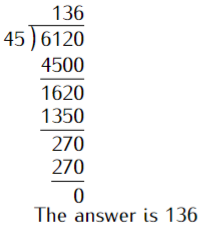
\includegraphics{Operations_Ex2.png}

}

\caption{Example 2}

\end{figure}

\end{tcolorbox}

\begin{tcolorbox}[enhanced jigsaw, leftrule=.75mm, opacityback=0, toprule=.15mm, bottomrule=.15mm, breakable, title=\textcolor{quarto-callout-note-color}{\faInfo}\hspace{0.5em}{Example 3}, opacitybacktitle=0.6, titlerule=0mm, colframe=quarto-callout-note-color-frame, rightrule=.15mm, coltitle=black, colback=white, bottomtitle=1mm, toptitle=1mm, left=2mm, colbacktitle=quarto-callout-note-color!10!white, arc=.35mm]

The Amos family borrows \$ 20,880 to purchase a new car at a special 0\%
interest rate. The car dealer allows them 5 years to pay back the amount
they borrow and requires equal monthly payments. How much are their
monthly payments? \((2mks)\)

\end{tcolorbox}

\begin{tcolorbox}[enhanced jigsaw, leftrule=.75mm, opacityback=0, toprule=.15mm, bottomrule=.15mm, breakable, title=\textcolor{quarto-callout-caution-color}{\faFire}\hspace{0.5em}{Solution}, opacitybacktitle=0.6, titlerule=0mm, colframe=quarto-callout-caution-color-frame, rightrule=.15mm, coltitle=black, colback=white, bottomtitle=1mm, toptitle=1mm, left=2mm, colbacktitle=quarto-callout-caution-color!10!white, arc=.35mm]

Since there are 12 months in each year, they must make a total of
\(5\times12 = 60\), payments on the loan. Dividing \$ 20,880 by 60 will
result in the monthly payment:

\begin{figure}[H]

{\centering 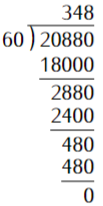
\includegraphics{Operations_Ex3.png}

}

\caption{Example 3}

\end{figure}

The Amos' monthly payment will be \$ 348.

\end{tcolorbox}

\begin{tcolorbox}[enhanced jigsaw, leftrule=.75mm, opacityback=0, toprule=.15mm, bottomrule=.15mm, breakable, title=\textcolor{quarto-callout-note-color}{\faInfo}\hspace{0.5em}{Problems to solve}, opacitybacktitle=0.6, titlerule=0mm, colframe=quarto-callout-note-color-frame, rightrule=.15mm, coltitle=black, colback=white, bottomtitle=1mm, toptitle=1mm, left=2mm, colbacktitle=quarto-callout-note-color!10!white, arc=.35mm]

\begin{enumerate}
\def\labelenumi{\arabic{enumi}.}
\item
  A bus charges \(Ksh.~ 150\) as fare from Embu to Meru. It carries a
  capacity of 18 passengers. However, it can carry 5 more passengers but
  will have to pay a penalty of \(Ksh.~100\) at each of the 8 police
  checkpoints it passes through. The distance between the two towns is
  \(91 ~km\) and the cost of petrol is \(Ksh.~ 102\) per litre. If the
  bus uses 1 litre for every \(7~ km\), calculate;

  a) How much is gained if the bus does not overload? \((4mks)\)

  b) How much is lost if the bus overloads? \((4mks)\)
\item
  A vegetable vendor had 1,652 cabbages. He sold 835 cabbages on the
  first day and 326 cabbages on the second day. He added 413 cabbages to
  the remaining stock on the third day.

  a) How many cabbages did he have at the end? \((3mks)\)

  b) If he sold all the cabbages at an average cost of \(Ksh.~ 15\), how
  much money did he collect? \((1mk)\)
\item
  Perform the following divisions: \((6mks)\)

  a) \(2,668\div58\)

  b) \(867,594 \div 2,317\)

  c) \(0.0021\div 14\)
\item
  A bookshop had \(29,424\) exercise books which were packed in cartons.
  each carton contained \(24\) exercise books. The mass of an empty
  carton was 2 Kg and 11 Kg when full.

  a) How many cartons were there? \((1mk)\)

  b) What was the total mass of empty cartons? \((2mks)\)

  c) What was the total mass of the books alone? \((2mks)\)
\item
  The average mass of students in a class of 45 was 46 Kg at the
  beginning of the year. At the end of the that year, they had each
  gained 4 Kg. Calculate:

  a) Their total mass of the students at the end of the year. \((2mks)\)

  b) The difference between their total mass at the beginning and at the
  end of the year. \((2mks)\)
\item
  A matatu had 23 passengers at the beginning of the journey. Twelve
  passengers alighted at the first stop while 9 boarded. Six of those
  who boarded at the first stop alighted at the second stop and 12 got
  in. The matatu did not stop again up to the final destination. The
  charges from the starting point were Ksh. 50 up to the first stop,
  Ksh. 70 up to the second stop, and Ksh. 85 up to the final
  destination.

  a) How many passengers alighted at the final destination? (3mks)

  b) How many passengers were carried by the matatu through the journey?
  (2mks)

  c) How much money was collected during the trip? (5mks)
\item
  a) State the value of digit 7 after the operations below.

  i) \(3.45 \times 20.54\) (2mks)

  ii) \(0.345 \times 2.054\) (2mks)

  iii) \(34.5\times 0.2054\) (2mks)

  iv) \(0.0345\times 2.054\) (2mks)

  b) states the value of the second digit in the product 675
  \times 44.4. (2mks)
\end{enumerate}

\end{tcolorbox}

\bookmarksetup{startatroot}

\hypertarget{chapter-2-factors}{%
\chapter{Chapter 2: Factors}\label{chapter-2-factors}}

\bookmarksetup{startatroot}

\hypertarget{factors}{%
\chapter*{Factors}\label{factors}}
\addcontentsline{toc}{chapter}{Factors}

\markboth{Factors}{Factors}

Factors are all numbers that divide a given number without leaving a
remainder.

\begin{tcolorbox}[enhanced jigsaw, leftrule=.75mm, opacityback=0, toprule=.15mm, bottomrule=.15mm, breakable, title=\textcolor{quarto-callout-note-color}{\faInfo}\hspace{0.5em}{Example of Factors}, opacitybacktitle=0.6, titlerule=0mm, colframe=quarto-callout-note-color-frame, rightrule=.15mm, coltitle=black, colback=white, bottomtitle=1mm, toptitle=1mm, left=2mm, colbacktitle=quarto-callout-note-color!10!white, arc=.35mm]

\begin{figure}[H]

{\centering 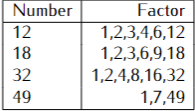
\includegraphics{Factor_Table.png}

}

\caption{Example}

\end{figure}

\end{tcolorbox}

\hypertarget{solved-examples-3}{%
\section{Solved examples}\label{solved-examples-3}}

\begin{tcolorbox}[enhanced jigsaw, leftrule=.75mm, opacityback=0, toprule=.15mm, bottomrule=.15mm, breakable, title=\textcolor{quarto-callout-note-color}{\faInfo}\hspace{0.5em}{Example 1}, opacitybacktitle=0.6, titlerule=0mm, colframe=quarto-callout-note-color-frame, rightrule=.15mm, coltitle=black, colback=white, bottomtitle=1mm, toptitle=1mm, left=2mm, colbacktitle=quarto-callout-note-color!10!white, arc=.35mm]

Express the following numbers in terms of their prime factors

a) 150 \((2mks)\)

b) 196 \((2mks)\)

\end{tcolorbox}

\begin{tcolorbox}[enhanced jigsaw, leftrule=.75mm, opacityback=0, toprule=.15mm, bottomrule=.15mm, breakable, title=\textcolor{quarto-callout-caution-color}{\faFire}\hspace{0.5em}{Solution}, opacitybacktitle=0.6, titlerule=0mm, colframe=quarto-callout-caution-color-frame, rightrule=.15mm, coltitle=black, colback=white, bottomtitle=1mm, toptitle=1mm, left=2mm, colbacktitle=quarto-callout-caution-color!10!white, arc=.35mm]

\begin{figure}[H]

{\centering 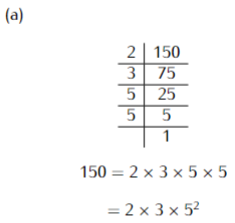
\includegraphics{Factor_Ex1_a.png}

}

\caption{Example 1 (a)}

\end{figure}

\begin{figure}[H]

{\centering 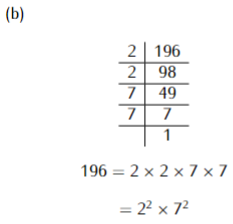
\includegraphics{Factor_Ex1_b.png}

}

\caption{Example 1 (b)}

\end{figure}

\end{tcolorbox}

\begin{tcolorbox}[enhanced jigsaw, leftrule=.75mm, opacityback=0, toprule=.15mm, bottomrule=.15mm, breakable, title=\textcolor{quarto-callout-note-color}{\faInfo}\hspace{0.5em}{Problems to solve}, opacitybacktitle=0.6, titlerule=0mm, colframe=quarto-callout-note-color-frame, rightrule=.15mm, coltitle=black, colback=white, bottomtitle=1mm, toptitle=1mm, left=2mm, colbacktitle=quarto-callout-note-color!10!white, arc=.35mm]

Express the following numbers in terms of their prime factors:

a) 1859 \hspace{11.2cm} \((2mks)\)

b) 105 \hspace{11.4cm} \((2mks)\)

c) 900 \hspace{11.4cm} \((2mks)\)

d) 700 \hspace{11.4cm} \((2mks)\)

e) 5929 \hspace{11.4cm} \((2mks)\)

f) 1078 \hspace{11.4cm} \((2mks)\)

g) 2057 \hspace{11.4cm} \((2mks)\)

h) 1386 \hspace{11.4cm} \((2mks)\)

i) 1573 \hspace{11.4cm} \((2mks)\)

j) 993 \hspace{11.4cm} \((2mks)\)

\end{tcolorbox}

\bookmarksetup{startatroot}

\hypertarget{chapter-three-divisibility-test}{%
\chapter{Chapter Three: Divisibility
Test}\label{chapter-three-divisibility-test}}

\bookmarksetup{startatroot}

\hypertarget{divisibility-test}{%
\chapter*{Divisibility Test}\label{divisibility-test}}
\addcontentsline{toc}{chapter}{Divisibility Test}

\markboth{Divisibility Test}{Divisibility Test}

\hypertarget{divisibility-test-for-2-3-4-5-6-8-10-and-11}{%
\section{Divisibility Test for 2, 3, 4, 5, 6, 8, 10, and
11}\label{divisibility-test-for-2-3-4-5-6-8-10-and-11}}

\textbf{Divisibility test for 2}

A number is divisible by \textbf{2} if its last digit is \textbf{even or
zero} . e.g., 12, 10, and 72

\textbf{Divisibility test for 3}

A number is divisible by \textbf{3} if the sum of its digits is
divisible by \textbf{3}.

\begin{tcolorbox}[enhanced jigsaw, leftrule=.75mm, opacityback=0, toprule=.15mm, bottomrule=.15mm, breakable, title=\textcolor{quarto-callout-note-color}{\faInfo}\hspace{0.5em}{Example}, opacitybacktitle=0.6, titlerule=0mm, colframe=quarto-callout-note-color-frame, rightrule=.15mm, coltitle=black, colback=white, bottomtitle=1mm, toptitle=1mm, left=2mm, colbacktitle=quarto-callout-note-color!10!white, arc=.35mm]

\(1,275\) is divisible by 3 because the sum of the digit is a multiple
of 3 that is:

\((1+2+7+5=15)=\frac{15}{3}=5\)

\end{tcolorbox}

\textbf{Divisibility test for 4}

A number is divisible by \textbf{4} if its last two digits are both zero
or form a number which is divisible by 4.

\begin{tcolorbox}[enhanced jigsaw, leftrule=.75mm, opacityback=0, toprule=.15mm, bottomrule=.15mm, breakable, title=\textcolor{quarto-callout-note-color}{\faInfo}\hspace{0.5em}{Example}, opacitybacktitle=0.6, titlerule=0mm, colframe=quarto-callout-note-color-frame, rightrule=.15mm, coltitle=black, colback=white, bottomtitle=1mm, toptitle=1mm, left=2mm, colbacktitle=quarto-callout-note-color!10!white, arc=.35mm]

\(1,144\) is divisible by 4 because its last two digits are divisible by
4 to give 11

\end{tcolorbox}

\textbf{Divisibility test for 5}

A number is divisible by 5 if its last digit is zero or 5. e.g 55, 60,
105

\textbf{Divisibility test for 6}

A number is divisible by 6 if it is divisible by both 2 and 3

\textbf{Divisibility test for 8}

A number is divisible by 8 if the number formed by its last 3 digits is
divisible by 8.

\textbf{Divisibility test for 9}

A number is divisible by 9 if the sum of its digits is divisible by 9

\textbf{Divisibility test for 10}

A number is divisible by 10 if the last digit is zero.

\textbf{Divisibility test for 11}

A number is divisible by 11 if the sum of its \textbf{1st, 3rd, 5th,
7th, 9th}, etc. digits and the sum of the 2nd, 4th, 6th, 8th, etc.
digits are equal or differ by 11 or a multiple of 11.

\begin{tcolorbox}[enhanced jigsaw, leftrule=.75mm, opacityback=0, toprule=.15mm, bottomrule=.15mm, breakable, title=\textcolor{quarto-callout-note-color}{\faInfo}\hspace{0.5em}{Problems to solve}, opacitybacktitle=0.6, titlerule=0mm, colframe=quarto-callout-note-color-frame, rightrule=.15mm, coltitle=black, colback=white, bottomtitle=1mm, toptitle=1mm, left=2mm, colbacktitle=quarto-callout-note-color!10!white, arc=.35mm]

\begin{enumerate}
\def\labelenumi{\arabic{enumi}.}
\item
  In each of the following numbers without doing actual division,
  determine whether the first number is divisible by the second number:
  \hspace{8.8 cm} \((5mks)\)

  a) 3409122; 6

  b) 17218; 6

  c) 11309634; ,8

  d) 515712; , 8

  e) 3501804; , 4
\item
  Which of the following numbers has 9 as a factor? \hspace{6cm}
  \((2mks)\)

  a) 394683

  b) 1872546

  c) 5172354
\item
  a) Which are the smallest numbers that can be added to the following
  numbers to make them divisible by 11? \hspace{10.8cm} \((4mks)\)

  i) 5,234

  ii) 36,541

  iii) 96,287

  iv) 27,992

  b) Which are the smallest numbers that can be subtracted from the
  following numbers to make them divisible by 11? \hspace{10cm}
  \((2mks)\)

  i) 96,287 ii) 24,535
\item
  Test whether 712,038 is divisible by: \hspace{8.5cm} \((3mks)\)

  i) 2

  ii) 3

  iii) 4
\end{enumerate}

\end{tcolorbox}

\bookmarksetup{startatroot}

\hypertarget{chapter-4-g.c.d-and-l.c.m}{%
\chapter{Chapter 4: G.C.D and L.C.M}\label{chapter-4-g.c.d-and-l.c.m}}

\bookmarksetup{startatroot}

\hypertarget{greatest-common-divisor-and-least-common-divisor}{%
\chapter*{Greatest Common Divisor and Least Common
Divisor}\label{greatest-common-divisor-and-least-common-divisor}}
\addcontentsline{toc}{chapter}{Greatest Common Divisor and Least Common
Divisor}

\markboth{Greatest Common Divisor and Least Common Divisor}{Greatest
Common Divisor and Least Common Divisor}

\hypertarget{greatest-common-divisor-gcd}{%
\section{Greatest Common Divisor
(GCD)}\label{greatest-common-divisor-gcd}}

GCD is also called the Highest Common Factor (HCF) or Greatest Common
Factor (GCF). To find the GCF of two numbers you write down their prime
factors, then select the common factors and obtain their product.

\begin{tcolorbox}[enhanced jigsaw, leftrule=.75mm, opacityback=0, toprule=.15mm, bottomrule=.15mm, breakable, title=\textcolor{quarto-callout-note-color}{\faInfo}\hspace{0.5em}{Solved Example}, opacitybacktitle=0.6, titlerule=0mm, colframe=quarto-callout-note-color-frame, rightrule=.15mm, coltitle=black, colback=white, bottomtitle=1mm, toptitle=1mm, left=2mm, colbacktitle=quarto-callout-note-color!10!white, arc=.35mm]

Find the HCF of 36 and 64. \hspace{10.5cm} \((3mks)\)

\end{tcolorbox}

\begin{tcolorbox}[enhanced jigsaw, leftrule=.75mm, opacityback=0, toprule=.15mm, bottomrule=.15mm, breakable, title=\textcolor{quarto-callout-caution-color}{\faFire}\hspace{0.5em}{Solution}, opacitybacktitle=0.6, titlerule=0mm, colframe=quarto-callout-caution-color-frame, rightrule=.15mm, coltitle=black, colback=white, bottomtitle=1mm, toptitle=1mm, left=2mm, colbacktitle=quarto-callout-caution-color!10!white, arc=.35mm]

\begin{figure}[H]

{\centering 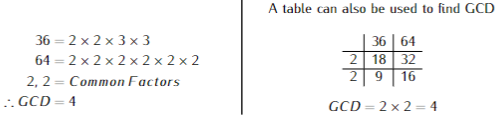
\includegraphics{GCD_Ex1.png}

}

\caption{GCD Example}

\end{figure}

\end{tcolorbox}

\hypertarget{least-common-multiple-lcm}{%
\section{Least Common Multiple (LCM)}\label{least-common-multiple-lcm}}

The least common multiple, or smallest common multiple, or lowest common
multiple of two integers is the smallest positive integer that is
divisible by the two integers.

\hypertarget{solved-examples-4}{%
\section{Solved Examples}\label{solved-examples-4}}

\begin{tcolorbox}[enhanced jigsaw, leftrule=.75mm, opacityback=0, toprule=.15mm, bottomrule=.15mm, breakable, title=\textcolor{quarto-callout-note-color}{\faInfo}\hspace{0.5em}{Example 1}, opacitybacktitle=0.6, titlerule=0mm, colframe=quarto-callout-note-color-frame, rightrule=.15mm, coltitle=black, colback=white, bottomtitle=1mm, toptitle=1mm, left=2mm, colbacktitle=quarto-callout-note-color!10!white, arc=.35mm]

What is the LCM of 18, 24 and 36? \hspace{9.5cm} \((2mks)\)

\end{tcolorbox}

\begin{tcolorbox}[enhanced jigsaw, leftrule=.75mm, opacityback=0, toprule=.15mm, bottomrule=.15mm, breakable, title=\textcolor{quarto-callout-caution-color}{\faFire}\hspace{0.5em}{Solution}, opacitybacktitle=0.6, titlerule=0mm, colframe=quarto-callout-caution-color-frame, rightrule=.15mm, coltitle=black, colback=white, bottomtitle=1mm, toptitle=1mm, left=2mm, colbacktitle=quarto-callout-caution-color!10!white, arc=.35mm]

\begin{figure}[H]

{\centering 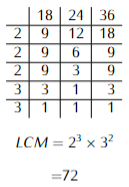
\includegraphics{GCD_LCM_Ex1.png}

}

\caption{Example 1}

\end{figure}

\end{tcolorbox}

\begin{tcolorbox}[enhanced jigsaw, leftrule=.75mm, opacityback=0, toprule=.15mm, bottomrule=.15mm, breakable, title=\textcolor{quarto-callout-note-color}{\faInfo}\hspace{0.5em}{Example 2}, opacitybacktitle=0.6, titlerule=0mm, colframe=quarto-callout-note-color-frame, rightrule=.15mm, coltitle=black, colback=white, bottomtitle=1mm, toptitle=1mm, left=2mm, colbacktitle=quarto-callout-note-color!10!white, arc=.35mm]

The G.C.D of two numbers is 12 and their L.C.M is 240. If one of the
numbers is 60, find the other number \hspace{14cm} \((3mks)\)

\end{tcolorbox}

\begin{tcolorbox}[enhanced jigsaw, leftrule=.75mm, opacityback=0, toprule=.15mm, bottomrule=.15mm, breakable, title=\textcolor{quarto-callout-caution-color}{\faFire}\hspace{0.5em}{Solution}, opacitybacktitle=0.6, titlerule=0mm, colframe=quarto-callout-caution-color-frame, rightrule=.15mm, coltitle=black, colback=white, bottomtitle=1mm, toptitle=1mm, left=2mm, colbacktitle=quarto-callout-caution-color!10!white, arc=.35mm]

\begin{figure}[H]

{\centering 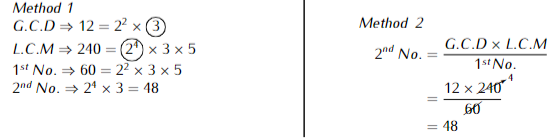
\includegraphics{GCD_LCM_Ex2.png}

}

\caption{Example 2}

\end{figure}

\end{tcolorbox}

\begin{tcolorbox}[enhanced jigsaw, leftrule=.75mm, opacityback=0, toprule=.15mm, bottomrule=.15mm, breakable, title=\textcolor{quarto-callout-note-color}{\faInfo}\hspace{0.5em}{Problems to solve}, opacitybacktitle=0.6, titlerule=0mm, colframe=quarto-callout-note-color-frame, rightrule=.15mm, coltitle=black, colback=white, bottomtitle=1mm, toptitle=1mm, left=2mm, colbacktitle=quarto-callout-note-color!10!white, arc=.35mm]

\begin{enumerate}
\def\labelenumi{\arabic{enumi}.}
\item
  The GCD of three numbers is 30 and their LCM is 900. Two of the
  numbers are 60 and 150. Find the other possible numbers.
  \hspace{8.7cm} \((3mks)\)
\item
  the least common multiple of two numbers is 60 and one of the numbers
  is 7 less than the other. What are the numbers? \hspace{10.3cm}
  \((3mks)\)
\item
  The L.C.M of two numbers is 120 and their G.C.F is 6. One of the
  numbers is 30, what is the other number? \hspace{11.8cm} \((3mks)\)
\item
  Three bells rang at intervals of 9minutes, 15 minutes and 21minutes.
  The bells will ring together at 11.00 p.m.Find the time the bells had
  last rang together. \hspace{5cm} \((3mks)\)
\item
  a) The difference between the GCD and the LCM of 36 and
  54.\hspace{4cm} \((2mks)\)

  b) If three numbers 36, 54 and have a GCD of 6 and LCM of 216. Find
  the least value of the third number. \hspace{11.1cm} \((2mks)\)
\item
  The GCD and LCM of three numbers are 3 and 1,008 respectively. If two
  of the numbers are 48 and 72, find the least possible value of the
  third number.\hspace{5cm} \((3mks)\)
\item
  Three alarms ring at intervals of 40 minutes, 45 minutes, and 60
  minutes. If they ring simultaneously at 6:30 a.m., at what time will
  they next ring together? \hspace{3.9cm} \((3mks)\)
\item
  Four traffic light signals are programmed at intervals of 40 seconds,
  50 seconds, 60 seconds, and 75 seconds. What is the earliest they will
  give out light signals simultaneously if the last time they did this
  was at 8:15 a.m.? \hspace{8.5cm} \((3mks)\)
\item
  A number n is such that when it is divided by 27, 30, or 45, the
  remainder is 5. Find the smallest possible value of n.~\hspace{11cm}
  \((3mks)\)
\item
  Find the greatest number which divides 181 and 170 leaving a remainder
  of 5. \hspace{1.7cm} \((3mks)\)
\item
  A square room is covered by a number of whole rectangular slabs of
  sides 60cm by 42 cm. Calculate the least possible area of the room in
  square meters. \hspace{4cm} \((3mks)\)
\item
  Three metal rods of lengths 234cm, 270cm, and 324cm were cut into
  shorter pieces all of the same length to make window grills. Calculate
  the length of the longest piece that can be cut from each of the rods
  and hence the total number of pieces that can be obtained from the
  rods. \hspace*\{14.2cm\} \((4mks)\)
\item
  The GCD of two numbers is 7 and their LCM is 140. If one of the
  numbers is 20, find the other number. \hspace{12.8cm} \((2mks)\)
\item
  The GCD and LCM of three numbers are 84 and 7056 respectively. If two
  of the numbers are 168 and 336, find the least possible value of the
  third number.\hspace{5cm} \((3mks)\)
\item
  A fruit juice dealer sells the juice in a packet of 300ml, 500ml, and
  750ml. Find the size of the smallest container that can fill each of
  the packets and leave a remainder of 200ml.\hspace{0.6cm} \((3mks)\)
\item
  Mr.~Ombogo the principal of Chiga secondary would wish to cover the
  floor of the new administration block using the square tiles. The
  floor is a rectangle of sides 12.8m by 8.4m. Find the area of each of
  the largest tiles which can be used to fit exactly without breaking.
  \hspace*\{14.2cm\} \((3mks)\)
\item
  Three numbers, 1400, 1960, and n have a G.C.D and L.C.M of 70 and
  \(2^2\times 5^2\times 7^2 \times 11\) respectively. Find the least
  possible value of n.~\hspace{8.8cm} \((3mks)\)
\item
  a) Express 48 and 60 as a product of their prime factors.
  \hspace{11cm} \((3mks)\)

  b) A room of sides 48m and 60m is to be decorated using square tiles
  side XM. Find the greatest area of the tile. \hspace{9.2cm} \((2mks)\)
\item
  Three similar pieces of timber of length 240cm, 320cm, and 380cm are
  cut into equal pieces. Find the largest possible area of a square that
  can be made from any of the three pieces. \hspace{14.2cm} \((3mks)\)
\end{enumerate}

\end{tcolorbox}

\bookmarksetup{startatroot}

\hypertarget{chapter-5-integers}{%
\chapter{Chapter 5: Integers}\label{chapter-5-integers}}

\bookmarksetup{startatroot}

\hypertarget{integers}{%
\chapter*{Integers}\label{integers}}
\addcontentsline{toc}{chapter}{Integers}

\markboth{Integers}{Integers}

\hypertarget{the-number-line}{%
\section{The Number Line}\label{the-number-line}}

Integers are positive whole numbers, negative whole numbers, and zero.
Integers are usually represented on the number line at equal intervals,
as shown in the figure below, where each interval is equal to one unit.

\begin{figure}

{\centering 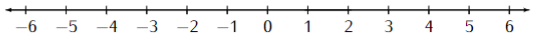
\includegraphics{Number_Line.png}

}

\caption{\label{fig-numberline}Number Line}

\end{figure}

Important properties to note while working with integers:

\begin{quote}
\textbf{Multiplication and division properties of integers}

\begin{itemize}
\item
  \((+)\times(-) = -\)
\item
  \((-) \times (+) = -\)
\item
  \((-) \times (-) = +\)
\item
  \((+) \times(+) = +\)
\item
  \((+)\div(-) = -\)
\item
  \((-)\div(+) = -\)
\item
  \((-)\div(-) = +\)
\end{itemize}
\end{quote}

\hypertarget{solved-examples-5}{%
\section{Solved Examples}\label{solved-examples-5}}

\begin{tcolorbox}[enhanced jigsaw, leftrule=.75mm, opacityback=0, toprule=.15mm, bottomrule=.15mm, breakable, title=\textcolor{quarto-callout-note-color}{\faInfo}\hspace{0.5em}{Example 1}, opacitybacktitle=0.6, titlerule=0mm, colframe=quarto-callout-note-color-frame, rightrule=.15mm, coltitle=black, colback=white, bottomtitle=1mm, toptitle=1mm, left=2mm, colbacktitle=quarto-callout-note-color!10!white, arc=.35mm]

Show how the following additions can be done using a number line and
give the results: \((6mks)\)

a) \((-4)+(+6)\)

b) \((-5)+(+4)\)

c) \((+2)+(-6)\)

\end{tcolorbox}

\begin{tcolorbox}[enhanced jigsaw, leftrule=.75mm, opacityback=0, toprule=.15mm, bottomrule=.15mm, breakable, title=\textcolor{quarto-callout-caution-color}{\faFire}\hspace{0.5em}{Solution}, opacitybacktitle=0.6, titlerule=0mm, colframe=quarto-callout-caution-color-frame, rightrule=.15mm, coltitle=black, colback=white, bottomtitle=1mm, toptitle=1mm, left=2mm, colbacktitle=quarto-callout-caution-color!10!white, arc=.35mm]

\begin{figure}[H]

{\centering 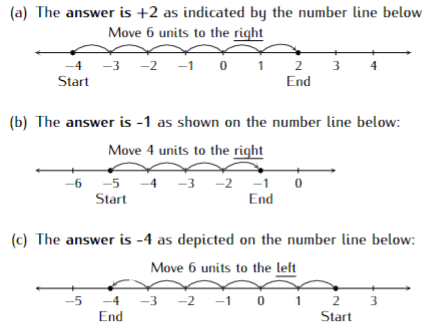
\includegraphics{Number_Line_ex1.png}

}

\caption{Example 1}

\end{figure}

\end{tcolorbox}

\begin{tcolorbox}[enhanced jigsaw, leftrule=.75mm, opacityback=0, toprule=.15mm, bottomrule=.15mm, breakable, title=\textcolor{quarto-callout-note-color}{\faInfo}\hspace{0.5em}{Example 2}, opacitybacktitle=0.6, titlerule=0mm, colframe=quarto-callout-note-color-frame, rightrule=.15mm, coltitle=black, colback=white, bottomtitle=1mm, toptitle=1mm, left=2mm, colbacktitle=quarto-callout-note-color!10!white, arc=.35mm]

Fill in the boxes in numbers below:\hspace{10cm} \((3mks)\)

i) \((-3)+\square=+10\)

ii) \(\square +(-7)=-11\)

iii) \((-4)+(-2)+\square =+3\)

\end{tcolorbox}

\begin{tcolorbox}[enhanced jigsaw, leftrule=.75mm, opacityback=0, toprule=.15mm, bottomrule=.15mm, breakable, title=\textcolor{quarto-callout-caution-color}{\faFire}\hspace{0.5em}{Solution}, opacitybacktitle=0.6, titlerule=0mm, colframe=quarto-callout-caution-color-frame, rightrule=.15mm, coltitle=black, colback=white, bottomtitle=1mm, toptitle=1mm, left=2mm, colbacktitle=quarto-callout-caution-color!10!white, arc=.35mm]

i) \(\square=+10+3=13\)

ii) \(\square=-11+7=-4\)

iii) \(\square-4-2=+3 \Rightarrow \square=3+6=+9\)

\end{tcolorbox}

\begin{tcolorbox}[enhanced jigsaw, leftrule=.75mm, opacityback=0, toprule=.15mm, bottomrule=.15mm, breakable, title=\textcolor{quarto-callout-note-color}{\faInfo}\hspace{0.5em}{Example 3}, opacitybacktitle=0.6, titlerule=0mm, colframe=quarto-callout-note-color-frame, rightrule=.15mm, coltitle=black, colback=white, bottomtitle=1mm, toptitle=1mm, left=2mm, colbacktitle=quarto-callout-note-color!10!white, arc=.35mm]

Without using a calculator evaluate, \hspace{10cm} \((3mks)\)

\[ 
\frac{-2(4+3)-12\div3 +2}{-6\times-3+-2\times4}
\]

\end{tcolorbox}

\begin{tcolorbox}[enhanced jigsaw, leftrule=.75mm, opacityback=0, toprule=.15mm, bottomrule=.15mm, breakable, title=\textcolor{quarto-callout-caution-color}{\faFire}\hspace{0.5em}{Solution}, opacitybacktitle=0.6, titlerule=0mm, colframe=quarto-callout-caution-color-frame, rightrule=.15mm, coltitle=black, colback=white, bottomtitle=1mm, toptitle=1mm, left=2mm, colbacktitle=quarto-callout-caution-color!10!white, arc=.35mm]

\textbf{Using BODMAS}

\begin{split}
 Numerator &=2(4+3)-12\div3+2\\
&=14-4+2\\
&=12\\
Denominator&=-6\times-3+ -2\times4 \\
&=18+-8\\
&=10\\
\therefore
&=\frac{12}{10}=\frac{6}{5}=1 \frac{1}{5}\\
\end {split}

\end{tcolorbox}

\begin{tcolorbox}[enhanced jigsaw, leftrule=.75mm, opacityback=0, toprule=.15mm, bottomrule=.15mm, breakable, title=\textcolor{quarto-callout-note-color}{\faInfo}\hspace{0.5em}{Problem to Solve}, opacitybacktitle=0.6, titlerule=0mm, colframe=quarto-callout-note-color-frame, rightrule=.15mm, coltitle=black, colback=white, bottomtitle=1mm, toptitle=1mm, left=2mm, colbacktitle=quarto-callout-note-color!10!white, arc=.35mm]

\begin{enumerate}
\def\labelenumi{\arabic{enumi}.}
\tightlist
\item
  Without using a calculator, evaluate \hspace{9.65cm} \((3mks)\).
\end{enumerate}

\[\frac{(-8+(-5)\times(-8)-(-6)}{-3+(-8)\div2\times4} \]

\begin{enumerate}
\def\labelenumi{\arabic{enumi}.}
\setcounter{enumi}{1}
\item
  Orengo bought 1848 Mangoes on a Wednesday and sold 650 of them on the
  same day. On Thursday, he sold 180 more Mangoes than on Wednesday. On
  Friday he bought 460 more Mangoes. Later that day, he sold all the
  Mangoes he had at a price of Ksh. 10 each. How much money did he make?
  \hspace{12cm} \((3mks)\)
\item
  Evaluate: \hspace{10.3cm} \((3mks)\)
\end{enumerate}

\[\frac{-12\div(-3)\times4-(-20)}{-6\times6\div+(-6)} \]

\begin{enumerate}
\def\labelenumi{\arabic{enumi}.}
\setcounter{enumi}{3}
\tightlist
\item
  Without using tables or a calculator, evaluate \hspace{6.85cm}
  \((3mks)\)
\end{enumerate}

\[ \frac{(-2)\times 7+(-4) \div (-3)}{3 \times (-2)+5\times (-4)}\]

\begin{enumerate}
\def\labelenumi{\arabic{enumi}.}
\setcounter{enumi}{4}
\tightlist
\item
  Without using a calculator, evaluate \hspace{10.7cm} \((3mks)\)\\
\end{enumerate}

\[\frac{-5(-23+41)-(-10)}{-3+(-8)\div2\times4}\]

\begin{enumerate}
\def\labelenumi{\arabic{enumi}.}
\setcounter{enumi}{5}
\item
  Show how the following additions can be done using a number line and
  give the results:

  a) \((-8)+(+5)\) \hspace{12cm} \((2mks)\)

  b) \((-7)+(+2)\) \hspace{12cm} \((2mks)\)

  c) \((-6)+(+4)+(+2)\) \hspace{10.95cm} \((2mks)\)
\end{enumerate}

\end{tcolorbox}

\bookmarksetup{startatroot}

\hypertarget{chapter-6-fractions}{%
\chapter{Chapter 6: Fractions}\label{chapter-6-fractions}}

\bookmarksetup{startatroot}

\hypertarget{fractions}{%
\chapter*{Fractions}\label{fractions}}
\addcontentsline{toc}{chapter}{Fractions}

\markboth{Fractions}{Fractions}

A fraction is written in the form of \(\frac{x}{y}\) where \(x\) and
\(y\) are numbers and \(y\neq0\). The number on the upper side \((x)\)
is called numerator and the number on the lower side \((y)\) is called
Denominator.

There are three types of fractions:

\begin{itemize}
\item
  \textbf{Proper fractions:} These are fractions whose numerator is
  smaller than the denominator.
\item
  \textbf{Improper fractions:} These are the fractions whose numerator
  is bigger than the denominator
\item
  \textbf{Mixed fractions:} They are fractions written in the form of an
  integer and a proper fraction.
\end{itemize}

\hypertarget{solved-examples-6}{%
\section{Solved Examples}\label{solved-examples-6}}

\begin{tcolorbox}[enhanced jigsaw, leftrule=.75mm, opacityback=0, toprule=.15mm, bottomrule=.15mm, breakable, title=\textcolor{quarto-callout-note-color}{\faInfo}\hspace{0.5em}{Example 1}, opacitybacktitle=0.6, titlerule=0mm, colframe=quarto-callout-note-color-frame, rightrule=.15mm, coltitle=black, colback=white, bottomtitle=1mm, toptitle=1mm, left=2mm, colbacktitle=quarto-callout-note-color!10!white, arc=.35mm]

Evaluate: \hspace{9cm} \((3mks)\)

\[
\frac{8\times \frac{1}{3} \, of\, 9\div 2-\frac{2}{3}\, of \,144 \div 12+2 \times 3}{\frac{3}{4}\, of \,36 \div 3-4\div \frac{2}{5} \,of \,10+3 \times (-2)}  
\]

\end{tcolorbox}

\begin{tcolorbox}[enhanced jigsaw, leftrule=.75mm, opacityback=0, toprule=.15mm, bottomrule=.15mm, breakable, title=\textcolor{quarto-callout-caution-color}{\faFire}\hspace{0.5em}{Solution}, opacitybacktitle=0.6, titlerule=0mm, colframe=quarto-callout-caution-color-frame, rightrule=.15mm, coltitle=black, colback=white, bottomtitle=1mm, toptitle=1mm, left=2mm, colbacktitle=quarto-callout-caution-color!10!white, arc=.35mm]

\textbf{Using BODMAS}

\begin{split}
Numerator: 
&=8\times \left(\frac{1}{3}\times9\right)\div 2-\left (\frac{2}{3}\times144\right)\div12+2\times3\\
&=8\times(3\div 2)-(96\div 12)+2 \times 3\\  
&=\left (8 \times \frac{3}{2}\right)-8+(2\times 3)\\
&=12-8+6\\
&=10\\
\end{split}

\begin{split}
Denominator:
&=\left( \frac{3}{4}\times36\right)\div 3-4\div\left (\frac{2}{5}\times10\right)+3\times(-2)\\
&=(27\div3)-(4\div4)+3\times-2\\
&=9-1+(3\times-2)\\
&=9-1-6\\
&=2\\
\therefore \frac{10}{2} &=5
\end{split}

\end{tcolorbox}

\begin{tcolorbox}[enhanced jigsaw, leftrule=.75mm, opacityback=0, toprule=.15mm, bottomrule=.15mm, breakable, title=\textcolor{quarto-callout-note-color}{\faInfo}\hspace{0.5em}{Example 2}, opacitybacktitle=0.6, titlerule=0mm, colframe=quarto-callout-note-color-frame, rightrule=.15mm, coltitle=black, colback=white, bottomtitle=1mm, toptitle=1mm, left=2mm, colbacktitle=quarto-callout-note-color!10!white, arc=.35mm]

James withdrew some money from a bank. He spent \(\frac{3}{8}\) of the
money to pay for his son's school fees and \(\frac{2}{5}\) to pay for
his daughter's school fees. If he remained with \(Ksh. 12, 330\),
calculate the amount of money he paid for his daughter's school fees.
\hspace{9.7cm} \((3mks)\)

\end{tcolorbox}

\begin{tcolorbox}[enhanced jigsaw, leftrule=.75mm, opacityback=0, toprule=.15mm, bottomrule=.15mm, breakable, title=\textcolor{quarto-callout-caution-color}{\faFire}\hspace{0.5em}{Solution}, opacitybacktitle=0.6, titlerule=0mm, colframe=quarto-callout-caution-color-frame, rightrule=.15mm, coltitle=black, colback=white, bottomtitle=1mm, toptitle=1mm, left=2mm, colbacktitle=quarto-callout-caution-color!10!white, arc=.35mm]

\begin{split}
Let\,his\, money\, be \,x \\
Son's\,school\, fees &= \frac{3}{8}x \\
Daughter's \,school\, fees&=\frac{2}{5}x \\
Remaining \,fraction&=x-\left( \frac{3}{8}x+\frac{2}{5}x\right)\\ x-\left ( \frac{31}{40}x\right) &=\frac{9}{40}x\\ 
\end{split}

\begin{split}
\frac{9}{40}x&=12330\\ multiply\: both \:sides \:by \:\frac{40}{9}\\ \therefore \frac{\cancel{40}}{\cancel9}\times\frac{\cancel9}{\cancel{40}}x&=12330\times\frac{40}{9}\\
x&=54800\\
Daughter's\, school \,fees&=\left (\frac{2}{5}\right) \times54800\\
&=Ksh. \,21,920
\end{split}

\end{tcolorbox}

\begin{tcolorbox}[enhanced jigsaw, leftrule=.75mm, opacityback=0, toprule=.15mm, bottomrule=.15mm, breakable, title=\textcolor{quarto-callout-note-color}{\faInfo}\hspace{0.5em}{Example 3}, opacitybacktitle=0.6, titlerule=0mm, colframe=quarto-callout-note-color-frame, rightrule=.15mm, coltitle=black, colback=white, bottomtitle=1mm, toptitle=1mm, left=2mm, colbacktitle=quarto-callout-note-color!10!white, arc=.35mm]

In a certain church, there are 200 more women than men. One-third of the
men and two-fifths of the women are elderly people. If there are 300
elderly people in the meeting, find out how many young people attend the
church.\hspace{12.1cm} \((3mks)\)

\end{tcolorbox}

\begin{tcolorbox}[enhanced jigsaw, leftrule=.75mm, opacityback=0, toprule=.15mm, bottomrule=.15mm, breakable, title=\textcolor{quarto-callout-caution-color}{\faFire}\hspace{0.5em}{Solution}, opacitybacktitle=0.6, titlerule=0mm, colframe=quarto-callout-caution-color-frame, rightrule=.15mm, coltitle=black, colback=white, bottomtitle=1mm, toptitle=1mm, left=2mm, colbacktitle=quarto-callout-caution-color!10!white, arc=.35mm]

\begin{split}
Let\, \,men&=x\\
women&=x+200\\
Elderly \,people&=300\\
\frac{1}{3}x+\frac{2}{5}(x+200)&=300\\
\frac{1}{3}x+\frac{2}{5}x+80&=300\\ 
\end{split}

\begin{split}
\frac{11}{15}x&=220\\
\frac{\cancel{15}}{\cancel{11}}\times \frac{\cancel{11}}{\cancel{15}}x&=\cancelto{20}{220}\times \frac{15}{\cancel{11}}\\
x&=20\times15\\&=300\,men\\ 
Total\, number \,of\, people:\\ men + women&=300+300+200\\&=800\\
young \,people&=800-300\\&=500\\
\end{split}

\end{tcolorbox}

\begin{tcolorbox}[enhanced jigsaw, leftrule=.75mm, opacityback=0, toprule=.15mm, bottomrule=.15mm, breakable, title=\textcolor{quarto-callout-note-color}{\faInfo}\hspace{0.5em}{Problems to solve}, opacitybacktitle=0.6, titlerule=0mm, colframe=quarto-callout-note-color-frame, rightrule=.15mm, coltitle=black, colback=white, bottomtitle=1mm, toptitle=1mm, left=2mm, colbacktitle=quarto-callout-note-color!10!white, arc=.35mm]

\begin{enumerate}
\def\labelenumi{\arabic{enumi}.}
\item
  Three people Karimi, Omondi, and Ali contributed money to start a
  business. Karimi contributed a quarter of the total amount and Omondi
  two-fifths of the remainder. Ali's contribution was one and a half
  times that of Karimi. They borrowed the rest of the money from the
  bank which was \(Ksh.\, 60, 000\) less than Ali's contribution, find
  the total amount required to start the business. \hspace{14.3cm}
  \((4mks)\)
\item
  Three people Gatungo, Martin, and Albert contributed money to purchase
  a flour mill. Gatungo contributed \(\frac{1}{3}\) of the total amount,
  Martin contributed \(\frac{3}{8}\) of the remaining amount and Albert
  contributed the rest of the money. The difference in contribution
  between Martin and Albert was \(Ksh. \,40, 000\). Calculate the price
  of the flour mill. \hspace{6cm} \((3mks)\)
\item
  Agnes paid rent which was \(\frac{1}{10}\) of her net salary. She used
  \(\frac{1}{2}\) of the remaining amount to make a down payment for a
  plot. She gave her mother \(Ksh.\, 2,500\) and did shopping worth
  \(Ksh.\, 7,500\) for herself. She saved the remainder which was
  \(Ksh.\, 12,500\). How much was the down payment that she made?
  \hspace{11.9cm} \((4mks)\)
\item
  King'oo spends one-third of his salary on food, one-quarter on rent,
  three--fifths of the remainder on transport, and saves the rest. If he
  spends \(Ksh. \,1,800\) on transport, find how much money he
  saves.\hspace{13.3cm} \((3mks)\)
\item
  Without using a calculator or mathematical table evaluate:
  \hspace{5.3cm} \((3mks)\)
\end{enumerate}

\[
\frac{2\frac{1}{5}+\frac{2}{3}\,of\,3\frac{3}{4}-4\frac{1}{6}}{1\frac{1}{4}+2\frac{2}{5}\div 1\frac{1}{3}+3\frac{3}{4}}  
\] 6. Without using a calculator, evaluate \hspace{11.5cm} \((3mks)\)

\[
\frac{\frac{3}{4}+1\frac{5}{7}\div \frac{4}{7}\,of\, 2\frac{1}{3}}{\left (1\frac{3}{7}-\frac{5}{8}\right)\times\frac{2}{3}}  
\] 7. Evaluate \hspace{9.5cm} \((3mks)\)

\[
\frac{\frac{3}{5}\,of\,60-2\frac{2}{3}\times1\frac{1}{2}}{5\frac{5}{8}\times1\frac{7}{9}-\frac{5}{4}\,of\,4\frac{4}{5}+2\frac{4}{5}\div\frac{7}{10}} 
\]

\begin{enumerate}
\def\labelenumi{\arabic{enumi}.}
\setcounter{enumi}{7}
\item
  Two boys and a girl shared some money. The younger boy \(\frac{5}{8}\)
  of it. The elder boy got \(\frac{7}{12}\) of the remainder and the
  girl got the rest. Find the percentage share of the younger boy to the
  girl's share. \hspace{13.2cm} \((2mks)\)
\item
  Evaluate without using a calculator. \((3mks)\)
\end{enumerate}

\[
\frac{\left( 2\frac{3}{7}-1\frac{5}{6}\right)\div\frac{5}{6}}{\frac{2}{3}\,of\,2\frac{1}{4}-1\frac{1}{7}} \hspace{12cm}
\]

\begin{enumerate}
\def\labelenumi{\arabic{enumi}.}
\setcounter{enumi}{9}
\tightlist
\item
  Evaluate: \((3mks)\)
\end{enumerate}

\[
\frac{\sqrt[]{\frac{1}{4}}\,of\,3\frac{1}{2}+\frac{3}{2}\left(\frac{5}{2}-\frac{2}{3}\right)}{\frac{3}{4}\,of\,2\frac{1}{2}\div\frac{1}{4}} \hspace{10.8cm} 
\]

\begin{enumerate}
\def\labelenumi{\arabic{enumi}.}
\setcounter{enumi}{10}
\tightlist
\item
  Without using a calculator, evaluate: \((3mks)\)
\end{enumerate}

\[
\frac{1\frac{4}{5}\,of\,\frac{25}{18}\div1\frac{2}{3}\times24}{2\frac{1}{3}-\frac{1}{4}\,of\,12\div\frac{5}{3}}  \hspace{11.2cm}    
\]

\begin{enumerate}
\def\labelenumi{\arabic{enumi}.}
\setcounter{enumi}{11}
\item
  Evaluate \hspace{12.8cm} \((6mks)\)

  a)
  \[\frac{5\frac{3}{5}\times 1\frac{3}{4}+8\frac{1}{3} \div \frac{5}{9}}{5\frac{1}{6}\times 1\frac{1}{5}}\]

  b)
  \[\frac{8\frac{2}{5}-3\frac{2}{3}\div 1\frac{5}{6}}{1\frac{1}{5}+ 1\frac{1}{3}\times 1\frac{1}{2}}\]
\item
  A man spent \(\frac{1}{9}\) his salary on food and \(\frac{1}{4}\) the
  remainder on electricity and water bills. He paid fees with \(20\%\)
  of his salary and invested \(16\%\) of what was left on business.\\
  After taking a game drive on which he spent \(Ksh. \,2,000\), he saved
  \(Ksh.\,5,350\). Calculate his monthly earnings. \((3mks)\)
\item
  In a mixed secondary school there are 60 more boys than girls. Half of
  the boys and \(\frac{2}{3}\) of the girls are boarders. If there are
  240 boarders, find the total number of students in the school.
  \hspace{14.2cm} \((3mks)\)
\item
  Five members of `SILK', a self-supporting enterprise Jane, Jepchoge,
  Esther, Mama Charo, and Chepkoech were given a certain amount of money
  to share amongst themselves.Jane got \(\frac{3}{8}\) of the total
  amount while Jepchoge got \(\frac{2}{5}\) of the remainder.The
  remaining amount was shared equally among Esther, Mama Charo, and
  Chepkoech each of which received \(Ksh.\, 6,000\);

  a) How much was shared among the five businesswomen? \hspace{4.3cm}
  \((3mks)\)

  b) How much did Jepchoge get? \hspace{8.5cm} \$(2mks)\$

  c) Jane, Jepchoge, and Chepkoech invested their money and earned a
  profit of \(Ksh.\, 12,000\). A third of the profit was left to
  maintain the business and the rest was shared according to their
  investments. Find how much each got.\hspace{6.5cm} \((5mks)\)
\end{enumerate}

\end{tcolorbox}

\bookmarksetup{startatroot}

\hypertarget{chapter-seven-decimals-squares-and-square-roots}{%
\chapter{Chapter Seven: Decimals, Squares, and Square
Roots}\label{chapter-seven-decimals-squares-and-square-roots}}

\bookmarksetup{startatroot}

\hypertarget{decimals-squares-and-square-roots}{%
\chapter*{Decimals, Squares, and Square
Roots}\label{decimals-squares-and-square-roots}}
\addcontentsline{toc}{chapter}{Decimals, Squares, and Square Roots}

\markboth{Decimals, Squares, and Square Roots}{Decimals, Squares, and
Square Roots}

\textbf{Decimal fraction} (Decimal), is a fraction whose denominator can
be written as a power of \(10\),
e.g.\(\frac{1}{10},\,\frac{3}{100}, and\,\frac{50}{100}\).

Decimal fractions are usually written in a special way, e.g.,
\(\frac{3}{10}\) written as \(0.3\). The dot in this notation is called
the \textbf{decimal point}. A decimal fraction that represents the sum
of a whole number and a proper fraction is called a \textbf{mixed
decimal}. In division, a decimal fraction in which a digit or a group of
digits repeat continuously without ending is called a \textbf{recurring
decimal} e.g.~\(\frac{5}{11}\)= 0.4545\ldots, in short, we place dots
above the digits that recurs e.g.~0.4545\ldots written as
\(0.\dot{4}\dot{5}\) A number is said to be in \textbf{standard form} if
it is expressed in the form \(A\times 10^n\) where \(1\leq A<10\) and
\(n\) is an integer e.g.~\(0.0065\) is written in standard form as
\(6.5\times 10^{-3}\).

\textbf{Squares} of numbers are tabulated and can be read from the table
of squares which gives only approximate values of the square to four
figures.

\textbf{Square root} of a number can be obtained using the factorization
method or tables of square roots in a mathematical table.

\hypertarget{solved-exambles}{%
\section{Solved Exambles}\label{solved-exambles}}

\begin{tcolorbox}[enhanced jigsaw, leftrule=.75mm, opacityback=0, toprule=.15mm, bottomrule=.15mm, breakable, title=\textcolor{quarto-callout-note-color}{\faInfo}\hspace{0.5em}{Example 1}, opacitybacktitle=0.6, titlerule=0mm, colframe=quarto-callout-note-color-frame, rightrule=.15mm, coltitle=black, colback=white, bottomtitle=1mm, toptitle=1mm, left=2mm, colbacktitle=quarto-callout-note-color!10!white, arc=.35mm]

Without using table or calculators, evaluate:

\[
\sqrt[]{\frac{0.0032+0.0608}{1.44\times 0.4}} \hspace{12cm} (3mks)
\]

\end{tcolorbox}

\begin{tcolorbox}[enhanced jigsaw, leftrule=.75mm, opacityback=0, toprule=.15mm, bottomrule=.15mm, breakable, title=\textcolor{quarto-callout-caution-color}{\faFire}\hspace{0.5em}{Solution}, opacitybacktitle=0.6, titlerule=0mm, colframe=quarto-callout-caution-color-frame, rightrule=.15mm, coltitle=black, colback=white, bottomtitle=1mm, toptitle=1mm, left=2mm, colbacktitle=quarto-callout-caution-color!10!white, arc=.35mm]

\begin{split}
0.0032+0.0608&=0.0640\\
1.44\times0.4&=0.576\\
\Rightarrow \sqrt[]{\frac{0.064\times1000}{0.576\times 1000}}&=\sqrt[]{\frac{64}{576}}
&=\frac{\sqrt[]{2^6}}{\sqrt[]{2^6\times3^2}}\\
&=\frac{\cancel{2^3}}{\cancel{2^3}\times 3}\\&=\frac{1}{3}
\end{split}

\end{tcolorbox}

\begin{tcolorbox}[enhanced jigsaw, leftrule=.75mm, opacityback=0, toprule=.15mm, bottomrule=.15mm, breakable, title=\textcolor{quarto-callout-note-color}{\faInfo}\hspace{0.5em}{Example 2}, opacitybacktitle=0.6, titlerule=0mm, colframe=quarto-callout-note-color-frame, rightrule=.15mm, coltitle=black, colback=white, bottomtitle=1mm, toptitle=1mm, left=2mm, colbacktitle=quarto-callout-note-color!10!white, arc=.35mm]

Express as a fraction:

\[
3.2\dot{5}\dot{6}  \hspace{14cm} (3mks)
\]

\end{tcolorbox}

\begin{tcolorbox}[enhanced jigsaw, leftrule=.75mm, opacityback=0, toprule=.15mm, bottomrule=.15mm, breakable, title=\textcolor{quarto-callout-caution-color}{\faFire}\hspace{0.5em}{Solution}, opacitybacktitle=0.6, titlerule=0mm, colframe=quarto-callout-caution-color-frame, rightrule=.15mm, coltitle=black, colback=white, bottomtitle=1mm, toptitle=1mm, left=2mm, colbacktitle=quarto-callout-caution-color!10!white, arc=.35mm]

\begin{split}
let \,r&=3.25656...& (i)&\\
10r&=32.5656... &(ii)&\\
100r&=325.656... &(iii)&\\
1000r&=3256.56... &(iv)&\\
\end{split}

\begin{split}
 &Subtracting \,(ii) \,from \,(iv)&\\
990r&=3224&\\r&=\frac{3224}{990}&\\
\therefore 3.2\dot{5}\dot{6}&=3\frac{127}{495}&
\end{split}

\end{tcolorbox}

\begin{tcolorbox}[enhanced jigsaw, leftrule=.75mm, opacityback=0, toprule=.15mm, bottomrule=.15mm, breakable, title=\textcolor{quarto-callout-note-color}{\faInfo}\hspace{0.5em}{Example 3}, opacitybacktitle=0.6, titlerule=0mm, colframe=quarto-callout-note-color-frame, rightrule=.15mm, coltitle=black, colback=white, bottomtitle=1mm, toptitle=1mm, left=2mm, colbacktitle=quarto-callout-note-color!10!white, arc=.35mm]

Use tables of square and square roots to evaluate.

\[
\sqrt[]{337.5}-\left(3.375\right)^2 \hspace{11.5cm} (3mks)
\]

\end{tcolorbox}

\begin{tcolorbox}[enhanced jigsaw, leftrule=.75mm, opacityback=0, toprule=.15mm, bottomrule=.15mm, breakable, title=\textcolor{quarto-callout-caution-color}{\faFire}\hspace{0.5em}{Solution}, opacitybacktitle=0.6, titlerule=0mm, colframe=quarto-callout-caution-color-frame, rightrule=.15mm, coltitle=black, colback=white, bottomtitle=1mm, toptitle=1mm, left=2mm, colbacktitle=quarto-callout-caution-color!10!white, arc=.35mm]

\begin{figure}[H]

{\centering 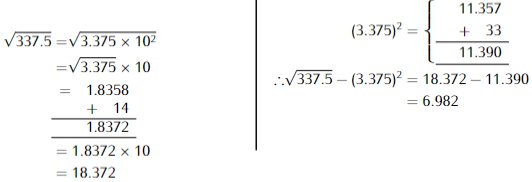
\includegraphics{Decimals_Ex3.png}

}

\caption{Example 3}

\end{figure}

\end{tcolorbox}

\begin{tcolorbox}[enhanced jigsaw, leftrule=.75mm, opacityback=0, toprule=.15mm, bottomrule=.15mm, breakable, title=\textcolor{quarto-callout-note-color}{\faInfo}\hspace{0.5em}{Problem to Solve}, opacitybacktitle=0.6, titlerule=0mm, colframe=quarto-callout-note-color-frame, rightrule=.15mm, coltitle=black, colback=white, bottomtitle=1mm, toptitle=1mm, left=2mm, colbacktitle=quarto-callout-note-color!10!white, arc=.35mm]

\begin{enumerate}
\def\labelenumi{\arabic{enumi}.}
\item
  Use the tables of squares and square roots only to find the value of:
  \[
  \left(0.0546\right)^{\frac{1}{2}} \hspace{12.1cm} (2mks)
  \]
\item
  Evaluate without using a calculator. \[
  \frac{23.4-2(5.2+5.3)}{3.2\times 1.2} \hspace{10.6cm} (3mks)
  \]
\item
  Use square tables to evaluate, to 4 significant figures. \[
  \left(8.254\right)^2 \hspace{12.5cm} (2mks)
  \]
\item
  Evaluate without using tables or calculator. \[
  \frac{2.5\times\sqrt[]{324}}{3\times\sqrt[]{729}} \hspace{12.4cm} (3mks)
  \]
\item
  Find the exact value of:\\
  \[
  2.\dot{4}\dot{1}-0.\dot{3}\dot{2} \hspace{12.2cm} (3mks)
  \]
\item
  The number \(5.\dot{8}\dot{1}\) contains an integral part and a
  recurring decimal. Convert the number into an improper fraction and
  hence a mixed fraction.\hspace{7cm} \((3mks)\)
\item
  Without using a calculator or mathematical tables find the value of:
  \[
  \frac{0.0060\times2.4\times0.3^2}{0.9\times0.00015\times160} \hspace{11cm} (3mks)
  \]
\item
  Express the recurring decimal below as a fraction;
  \(0.3\dot{7}\dot{2}\) leaving your answer in the form of
  \(\frac{a}{b}\) where \(a\) and \(b\) are integers.
\item
  Use the square and square-root tables to evaluate to 4 significant
  figures the expression. \[
  \left(43.46\right)^2-\sqrt[]{3785.4}\hspace{11.5cm} (4mks)
  \]
\item
  Using tables of square roots and reciprocals, evaluate : \[
  \sqrt[]{0.1964}+(0.478)^2\hspace{11.5cm} (3mks)
  \]
\item
  Convert \(0.63\dot{3}\dot{1}\) into a fraction without using a
  calculator. \hspace{4.75cm} \((3mks)\)
\item
  Use square and square root tables to calculate to 3 significant
  figures the value of: \[
  \sqrt[]{\left(0.04766\right)^2-(0.00972)^2} \hspace{10.1cm} (4mks)
  \]
\item
  Use square roots and square tables to evaluate the expression: \[
  \left(0.005467\right)^2+\left(0.04328\right)^2 \hspace{9.95cm} (3mks)
  \]
\item
  The surface area of a sphere of radius,r is given by the formula
  \(A = 4\pi r^2\). using square root tables, calculate the radius of
  the sphere whose surface area is \(120 cm^2\) \hspace{3.2cm} \$(3mks)
  \$
\item
  The periodic time for the swing of a pendulum in seconds is given by
  the formula,\(T =2\pi\sqrt[]{\frac{l}{g}}\). Using square root tables,
  calculate the value of \(T\) when \(l = 23.7cm\) and
  \(g = 1000 cms^{-2}\). \hspace*{14.2cm} \((3mks)\)
\end{enumerate}

\end{tcolorbox}

\bookmarksetup{startatroot}

\hypertarget{chapter-eight-algebraic-expressions}{%
\chapter{Chapter Eight: Algebraic
Expressions}\label{chapter-eight-algebraic-expressions}}

\bookmarksetup{startatroot}

\hypertarget{algebraic-expressions}{%
\chapter*{Algebraic Expressions}\label{algebraic-expressions}}
\addcontentsline{toc}{chapter}{Algebraic Expressions}

\markboth{Algebraic Expressions}{Algebraic Expressions}

\textbf{Algebraic expression}, is an expression built up from integer
constants, variables, and algebraic operations (Addition, subtraction,
division and multiplication).

\hypertarget{solved-problems}{%
\section{Solved problems}\label{solved-problems}}

\begin{tcolorbox}[enhanced jigsaw, leftrule=.75mm, opacityback=0, toprule=.15mm, bottomrule=.15mm, breakable, title=\textcolor{quarto-callout-note-color}{\faInfo}\hspace{0.5em}{Example 1}, opacitybacktitle=0.6, titlerule=0mm, colframe=quarto-callout-note-color-frame, rightrule=.15mm, coltitle=black, colback=white, bottomtitle=1mm, toptitle=1mm, left=2mm, colbacktitle=quarto-callout-note-color!10!white, arc=.35mm]

Simplify the following:

\end{tcolorbox}

\begin{tcolorbox}[enhanced jigsaw, leftrule=.75mm, opacityback=0, toprule=.15mm, bottomrule=.15mm, breakable, title=\textcolor{quarto-callout-note-color}{\faInfo}\hspace{0.5em}{Example 1 (a)}, opacitybacktitle=0.6, titlerule=0mm, colframe=quarto-callout-note-color-frame, rightrule=.15mm, coltitle=black, colback=white, bottomtitle=1mm, toptitle=1mm, left=2mm, colbacktitle=quarto-callout-note-color!10!white, arc=.35mm]

a) \[\frac{2m-am-2y+ay}{2m+2y-am-ay} \hspace{11cm} (3 mks)\]

\end{tcolorbox}

\begin{tcolorbox}[enhanced jigsaw, leftrule=.75mm, opacityback=0, toprule=.15mm, bottomrule=.15mm, breakable, title=\textcolor{quarto-callout-caution-color}{\faFire}\hspace{0.5em}{Solution}, opacitybacktitle=0.6, titlerule=0mm, colframe=quarto-callout-caution-color-frame, rightrule=.15mm, coltitle=black, colback=white, bottomtitle=1mm, toptitle=1mm, left=2mm, colbacktitle=quarto-callout-caution-color!10!white, arc=.35mm]

Factorizing the \textbf{Numerator:}

\begin{split}
2m-am-2y+ay&=m(2-a)-y(2-a)\\&=(m-y)(2-a)\\ 
\end{split}

Factorizing the \textbf{Denominator:}

\begin{split}
2m+2y-am-ay&=2(m+y)-a(m+y)\\&=(2-a)(m+y)\\  \\
\Rightarrow \, \frac{(m-y)\cancel{(2-a)})}{\cancel{(2-a)}(m+y)}&=\frac{(m-y)}{(m+y)}
\end{split}

\end{tcolorbox}

\begin{tcolorbox}[enhanced jigsaw, leftrule=.75mm, opacityback=0, toprule=.15mm, bottomrule=.15mm, breakable, title=\textcolor{quarto-callout-note-color}{\faInfo}\hspace{0.5em}{Example 1 (b)}, opacitybacktitle=0.6, titlerule=0mm, colframe=quarto-callout-note-color-frame, rightrule=.15mm, coltitle=black, colback=white, bottomtitle=1mm, toptitle=1mm, left=2mm, colbacktitle=quarto-callout-note-color!10!white, arc=.35mm]

b) \[\frac{x^2-4ax-4a+x}{(x+1)(4a^2-ax)} \hspace{11cm} (3 mks)\]

\end{tcolorbox}

\begin{tcolorbox}[enhanced jigsaw, leftrule=.75mm, opacityback=0, toprule=.15mm, bottomrule=.15mm, breakable, title=\textcolor{quarto-callout-caution-color}{\faFire}\hspace{0.5em}{Solution}, opacitybacktitle=0.6, titlerule=0mm, colframe=quarto-callout-caution-color-frame, rightrule=.15mm, coltitle=black, colback=white, bottomtitle=1mm, toptitle=1mm, left=2mm, colbacktitle=quarto-callout-caution-color!10!white, arc=.35mm]

Factorizing the \textbf{Numerator:}

\begin{split}
x^2-4ax-4a+x&=x(x-4a)+1(x-4a)\\ 
&=(x+1)(x-4a)\\ 
\end{split}

\textbf{Denominator:}

\begin{split}
(x+1)(4a^2-ax)\\
\Rightarrow \frac{\cancel{(x+1)}(x-4a)}{\cancel{(x+1)}(4a^2-ax)}&=\frac{x-4a}{a(4a-x)}&\\ 
&=\frac{\cancel{x-4a}}{-a(\cancel{x-4a)}}\\&=\frac{-1}{a}&
\end{split}

\end{tcolorbox}

\begin{tcolorbox}[enhanced jigsaw, leftrule=.75mm, opacityback=0, toprule=.15mm, bottomrule=.15mm, breakable, title=\textcolor{quarto-callout-note-color}{\faInfo}\hspace{0.5em}{Example 1 (c)}, opacitybacktitle=0.6, titlerule=0mm, colframe=quarto-callout-note-color-frame, rightrule=.15mm, coltitle=black, colback=white, bottomtitle=1mm, toptitle=1mm, left=2mm, colbacktitle=quarto-callout-note-color!10!white, arc=.35mm]

c) \[\frac{x-2y}{12p}-\frac{x+3y}{60p}  \hspace{11cm} (3 mks)\]

\end{tcolorbox}

\begin{tcolorbox}[enhanced jigsaw, leftrule=.75mm, opacityback=0, toprule=.15mm, bottomrule=.15mm, breakable, title=\textcolor{quarto-callout-caution-color}{\faFire}\hspace{0.5em}{Solution}, opacitybacktitle=0.6, titlerule=0mm, colframe=quarto-callout-caution-color-frame, rightrule=.15mm, coltitle=black, colback=white, bottomtitle=1mm, toptitle=1mm, left=2mm, colbacktitle=quarto-callout-caution-color!10!white, arc=.35mm]

\begin{split}
L.C.M&=60p\\ \frac{x-2y}{12p}-\frac{x+3y}{60p}&=\frac{5(x-2y)-(x+3y)}{60p}\\&=\frac{5x-10y-x-3y}{60p} \\
&=\frac{4x-13y}{60p}
\end{split}

\end{tcolorbox}

\begin{tcolorbox}[enhanced jigsaw, leftrule=.75mm, opacityback=0, toprule=.15mm, bottomrule=.15mm, breakable, title=\textcolor{quarto-callout-note-color}{\faInfo}\hspace{0.5em}{Example 2}, opacitybacktitle=0.6, titlerule=0mm, colframe=quarto-callout-note-color-frame, rightrule=.15mm, coltitle=black, colback=white, bottomtitle=1mm, toptitle=1mm, left=2mm, colbacktitle=quarto-callout-note-color!10!white, arc=.35mm]

Given that p=4, q=-3, and r=-1 find the value of:
\[\frac{2pqr^4+pqr-pr}{4pr-2qr+2pqr} \hspace{6cm} (3mks) \]

\end{tcolorbox}

\begin{tcolorbox}[enhanced jigsaw, leftrule=.75mm, opacityback=0, toprule=.15mm, bottomrule=.15mm, breakable, title=\textcolor{quarto-callout-caution-color}{\faFire}\hspace{0.5em}{Solution}, opacitybacktitle=0.6, titlerule=0mm, colframe=quarto-callout-caution-color-frame, rightrule=.15mm, coltitle=black, colback=white, bottomtitle=1mm, toptitle=1mm, left=2mm, colbacktitle=quarto-callout-caution-color!10!white, arc=.35mm]

\textbf{Numerator:}

\begin{split}
2pqr^4+pqr-pr&=2(4)(-3)(-1)^4+(4)(-3)(-1)-(4)(-1)&\\
&=-24+12+4\\&=-8\\
\end{split}

\textbf{Denominator:}

\begin{split}
4pr-2qr+2pqr&=4(4)(-1)-2(-3)(-1)+2(4)(-3)(-1)\\&=-16-6+24\\&=2\\
\therefore \frac{\cancelto{-4}{-8}}{\cancel2}&=-4
\end{split}

\end{tcolorbox}

\begin{tcolorbox}[enhanced jigsaw, leftrule=.75mm, opacityback=0, toprule=.15mm, bottomrule=.15mm, breakable, title=\textcolor{quarto-callout-note-color}{\faInfo}\hspace{0.5em}{Example 3}, opacitybacktitle=0.6, titlerule=0mm, colframe=quarto-callout-note-color-frame, rightrule=.15mm, coltitle=black, colback=white, bottomtitle=1mm, toptitle=1mm, left=2mm, colbacktitle=quarto-callout-note-color!10!white, arc=.35mm]

Simplify

\[\frac{(4a+b)^2-(b-4a)^2}{(a+b)^2-(b-a)^2} \hspace{13cm}  (4mks) \]

\end{tcolorbox}

\begin{tcolorbox}[enhanced jigsaw, leftrule=.75mm, opacityback=0, toprule=.15mm, bottomrule=.15mm, breakable, title=\textcolor{quarto-callout-caution-color}{\faFire}\hspace{0.5em}{Solution}, opacitybacktitle=0.6, titlerule=0mm, colframe=quarto-callout-caution-color-frame, rightrule=.15mm, coltitle=black, colback=white, bottomtitle=1mm, toptitle=1mm, left=2mm, colbacktitle=quarto-callout-caution-color!10!white, arc=.35mm]

\textbf{Numerator}:

\begin{split}
(4a+b)^2&=(4a+b)(4a+b)&\\
&=4a(4a+b)+b(4a+b)&\\&=16a^2+4ab+4ab+b^2&\\
&=16a^2+8ab+b^2&\\
 (b-4a)^2&=(b-4a)(b-4a)&\\&=b(b-4a)-4a(b-4a)&\\&=b^2-4ab-4ab+16a^2\\
&=b^2-8ab+16a^2&\\ 
(4a+b)^2-(b-4a)^2&=16a^2+8ab+b^2-(b^2-8ab+16a^2)\\
&=16a^2+8ab+b^2-b^2+8ab-16a^2&\\
&=8ab+8ab\\&=16ab&\\
\end{split}

\textbf{Denominator:}

\begin{split}
(a+b)^2&=(a+b)(a+b)&\\
&=a(a+b)+b(a+b)\\&=a^2+ab+ab+b^2&\\
&=a^2+2ab+b^2&\\
(b-a)^2&=(b-a)(b-a)&\\
&=b(b-a)-a(b-a)&\\&=b^2-ab-ab+a^2&\\
&=b^2-2ab+a^2&\\
(a+b)^2-(b-a)^2&=a^2+2ab+b^2-(b^2-2ab+a^2)&\\
&=a^2+2ab+b^2-b^2+2ab-a^2\\
&=2ab+2ab\\&=4ab&\\ 
\therefore \frac{\cancelto{4}{16ab}}{\cancel{4ab}}&=4&\\
\end{split}

\end{tcolorbox}

\begin{tcolorbox}[enhanced jigsaw, leftrule=.75mm, opacityback=0, toprule=.15mm, bottomrule=.15mm, breakable, title=\textcolor{quarto-callout-note-color}{\faInfo}\hspace{0.5em}{Example 4}, opacitybacktitle=0.6, titlerule=0mm, colframe=quarto-callout-note-color-frame, rightrule=.15mm, coltitle=black, colback=white, bottomtitle=1mm, toptitle=1mm, left=2mm, colbacktitle=quarto-callout-note-color!10!white, arc=.35mm]

Solve the equation\\
\[\frac{3}{2r}=\frac{5}{5r-1} \hspace{12cm}         (2mks)\]

\end{tcolorbox}

\begin{tcolorbox}[enhanced jigsaw, leftrule=.75mm, opacityback=0, toprule=.15mm, bottomrule=.15mm, breakable, title=\textcolor{quarto-callout-caution-color}{\faFire}\hspace{0.5em}{Solution}, opacitybacktitle=0.6, titlerule=0mm, colframe=quarto-callout-caution-color-frame, rightrule=.15mm, coltitle=black, colback=white, bottomtitle=1mm, toptitle=1mm, left=2mm, colbacktitle=quarto-callout-caution-color!10!white, arc=.35mm]

Multiply both sides by the L.C.M of the \textbf{denominator}

\begin{split}
L.C.M &=2r(5r-1)\\
\frac{3(\cancel{2r}(5r-1))}{\cancel{2r}}&=\frac{5(2r(\cancel{5r-1}))}{\cancel{5r-1}}\\
3(5r-1)&=5(2r)\\ 
15r-3&=10r\\
15r-10r&=3\\
\frac{\cancel5r}{\cancel5}&=\frac{3}{5}\\ \therefore r&=\frac{3}{5}\\
\end{split}

\end{tcolorbox}

\begin{tcolorbox}[enhanced jigsaw, leftrule=.75mm, opacityback=0, toprule=.15mm, bottomrule=.15mm, breakable, title=\textcolor{quarto-callout-note-color}{\faInfo}\hspace{0.5em}{Example 5}, opacitybacktitle=0.6, titlerule=0mm, colframe=quarto-callout-note-color-frame, rightrule=.15mm, coltitle=black, colback=white, bottomtitle=1mm, toptitle=1mm, left=2mm, colbacktitle=quarto-callout-note-color!10!white, arc=.35mm]

In fourteen years' time, a mother will be twice as old as her son. Four
years ago, the sum of their ages was 30 years. Find how old the mother
was when the son was born.\(\hspace{3 cm} (4 mks)\)

\end{tcolorbox}

\begin{tcolorbox}[enhanced jigsaw, leftrule=.75mm, opacityback=0, toprule=.15mm, bottomrule=.15mm, breakable, title=\textcolor{quarto-callout-caution-color}{\faFire}\hspace{0.5em}{Solution}, opacitybacktitle=0.6, titlerule=0mm, colframe=quarto-callout-caution-color-frame, rightrule=.15mm, coltitle=black, colback=white, bottomtitle=1mm, toptitle=1mm, left=2mm, colbacktitle=quarto-callout-caution-color!10!white, arc=.35mm]

\begin{split}
\underline{14 \,yrs \,time:} \\
Mother&=2x\\ son&=x\\
\underline{ Present\, age:}\\
Mother&=2x-14\\ Son&=x-14\\
\underline{4 \, yrs\, ago:}\\ 
Mother&=2x-14-4\\Son&=x-14-4\\ 
\end{split}

\begin{split}
\underline{Sum \,of\, their\, age:}\\
(2x-18)+(x-18)&=30\\3x-36&=30\\
\frac{\cancel{3}x}{\cancel{3}}&=\cancelto{\frac{22}{1}}{\frac{66}{3}}\\&=22, years\\ 
Mother \Rightarrow (44-14)&= 30 \,years\, now\\
Son \Rightarrow (22-14)&= 8 \,years\, now\\ Mother's\, age\, when\, giving \,birth&=30-8\\&=22\,years
\end{split}

\(\therefore\) The mother was 22 years old when the son was born.

\end{tcolorbox}

\begin{tcolorbox}[enhanced jigsaw, leftrule=.75mm, opacityback=0, toprule=.15mm, bottomrule=.15mm, breakable, title=\textcolor{quarto-callout-note-color}{\faInfo}\hspace{0.5em}{Problems to Solve}, opacitybacktitle=0.6, titlerule=0mm, colframe=quarto-callout-note-color-frame, rightrule=.15mm, coltitle=black, colback=white, bottomtitle=1mm, toptitle=1mm, left=2mm, colbacktitle=quarto-callout-note-color!10!white, arc=.35mm]

\begin{enumerate}
\def\labelenumi{\arabic{enumi}.}
\item
  Esther has \(26\) coins whose total value is \(Ksh.\,205\). There are
  thrice as many \(Ksh.\,10\) coins as there are \(Ksh.\,20\) coins. The
  rest are 50cts coins. Find the number of \(Ksh.\,20\) coins that
  Esther has. \(\hspace{13.9cm} (3mks)\)
\item
  Joyce has 21 coins whose total value is \(Ksh. \,72\). There are twice
  as many five shillings coins as there are ten shillings coins. The
  rest are one shilling coin. Find the number of ten shillings coins
  that Joyce has. \(\hspace{12 cm} (3 mks)\)
\item
  A rectangular plot is \(0.4 m\) longer than it is wide. If its length
  is \(6m\) find its perimeter. When the breadth of the rectangle is
  reduced by \(0.5m\), the length is increased such that the perimeter
  is increased by \(\frac{1}{4}\) of its original. What is the change in
  the length of the rectangle? \(\hspace{14.5 cm} (3 mks)\)
\item
  Three fruit vendors Musa, Florence, and Josephine agreed to share
  \(Ksh.\,1800\) gained after a sale of the property. For every
  \(Ksh.\, 1\) that Musa gets, Florence gets 50cts and for every
  \(Ksh.\,2\) that Florence gets Josephine gets \(Ksh.\,3\). Find
  Florence's share.\(\hspace{3.5 cm} (3mks)\)
\item
  Three-fifths of the work is done on the first day. On the second day,
  \(\frac{3}{4} \,\)of the remainder is completed. If on the third day
  \(\frac{7}{8} \,\)of what remained is done, what fraction of the work
  still remains to be done? \(\hspace{14.4 cm} (3mks)\)
\item
  Three years ago, Albina was three times as old as her son. In five
  years' time, the sum of their ages will be 76. Determine their present
  ages. \(\hspace{6.5cm} (3mks)\)
\item
  Simplify \(\hspace{13 cm} (3mks)\)
\end{enumerate}

\[\frac{(4p+2q)^2-(2q-4p)^2}{(2p+q)^2-(q-2p)^2} \]

\begin{enumerate}
\def\labelenumi{\arabic{enumi}.}
\setcounter{enumi}{7}
\item
  In a poultry farm, there are eight more hens than ducks, three times
  as many turkeys as hens, and three-quarters as many quails as turkeys.

  a) If there are x ducks, write down a simplified expression in x for
  the total number of birds on the farm. \(\hspace{12.9cm}(1mk)\)

  b) Find the total number of birds given that there are 162 quails.
  \(\hspace{3.4cm}(2mks)\)
\item
  Jane's mother is now four times as older than her. In eight years'
  time, she will be three times as old as her daughter. Find their
  present ages. \(\hspace{6.9cm} (3mks)\)
\item
  Factorize completely \(\hspace{11cm} (3mks)\)
\end{enumerate}

\[
(p-2q)(3p+2q)-(p-2q)^2
\] 11. Simplify the following expression by reducing it to a single
fraction \(\hspace{3.1cm} (3 mks)\)

\[
\frac{4p-3}{3}-\frac{3p-4}{4}=\frac{3-p}{6}
\]

\begin{enumerate}
\def\labelenumi{\arabic{enumi}.}
\setcounter{enumi}{11}
\item
  After work a hawker had four times as many ten-shilling coins as
  twenty-shilling coins, eight times as many five-shilling coins as
  twenty-shilling coins and thrice as many one-shilling coins as
  ten-shilling coins. After counting his money he found that he had a
  total of \(Ksh.\, 560\). Calculate the number of coins he had.
  \(\hspace{9.7cm} (3mks)\)
\item
  Osinya is now two times as old as his younger brother and three times
  as old as his son. Four years from now Osinya's age will be twelve
  years more than the sum of the ages of his son and younger brother.
  Find Osinya and his son present age.\(\hspace{5.5cm} (4mks)\)
\item
  Wathitha is now three times as old as Fatuma. Seven years ago Wathitha
  was exactly two-third times as old as Fatuma will be 14 years from
  now. Find Wathitha's present age. \(\hspace{1.3cm}(3mks)\)
\item
  Fadhili is now two and a half times as old as his son. Sixteen years
  ago his age was 7 years more than his son will be 7 years from now.
  Calculate Fadhili's present age. \(\hspace{2.9cm} (3mks)\)
\item
  In a church harambee meeting, there were 300 people present. Each man
  contributed \(Ksh. \,500\) and each woman \(Ksh.\, 300\). The meeting
  raised a total of \(Ksh.\, 100,200\). Calculate the number of men
  present in the meeting. \(\hspace{9.5cm} (3mks)\)
\item
  A group of 144 women and young girls in a certain church organized a
  trip to Kisumu. Each woman paid \(Ksh. \,900\) while each girl paid
  half as much. In this way the group raised a total of
  \(Ksh.\, 81,000\) for the trip. Calculate the number of women in the
  group. \(\hspace{2.4cm} (3mks)\)
\item
  The sum of age's three children of Awiti, Wafula, and Najala is 68
  years. Wafula is three-quarter as old as Awiti and twice times as old
  as Najala. Determine their ages. \(\hspace{2.8cm} (3mks)\)
\item
  Mwangi working on a coffee factory is paid \(Ksh.\, 40\) for every
  normal working hour and \(Ksh.\, 60\) for each hour worked overtime.
  During one week he worked for a total of 80 hours and was paid
  \(Ksh. \,3840\) in wages. Determine the number of hours he worked
  overtime. \(\hspace{1.2cm}(3mks)\)
\item
  A retailer has bought a mixture of bags of beans and bags of peas from
  a wholesaler. One bag of beans has a mass of 90 Kg and one bag of peas
  has a mass of 75 Kg. the retailer bought 350 bags whose total mass is
  28.5 tonnes. Find the number of bags of each type he bought.
  \(\hspace{-0cm} (3mks)\)
\item
  Given that \(x=4,\, y= -3 ,\, and \,\,z= -1\) evaluate.
  \(\hspace{7.5cm} (6mks)\)

  a) \[ \frac{2(x+z)^2-(x-y)(y-z)}{3(x+y)-2(y-z)}\]

  b) \[
  \frac{2xy^2-3xy^2z^2-3xy^2z}{x^2yz-2xyz^2-4xyz}
  \]
\item
  In a certain year, Waithera had 5 times as many goats as cows and
  three-quarter as many sheep as goats. In the next year the number of
  goats increased by 24\%, the number of cows decreased by 50\% while
  the number of sheep decreased by 30\%. At the end of the preceding
  year Waithera had a total of 1865 animals. Calculate to three
  significant figures the percentage decrease in the total number of
  animals during the preceding year. \(\hspace{5.6cm} (10mks)\)
\item
  A family has two children whose age difference is 9. Twice the sum of
  their ages is equal to the age of their father.

  a) By letting the age of the younger child be x, write an expression
  of the:

  i) Age of the elder child. \(\hspace{10.5 cm} (1mk)\)

  ii) Age of their father. \(\hspace{11 cm} (1mk)\)

  iii) If in 19 years' time, the product of the ages of the two children
  is equal to 14 times the age of their father; form an equation in x
  and hence determine the present possible age of the younger child.
  \(\hspace{13.6 cm} (4mks)\)

  iv) Determine the possible age of the elder child in 19 years' time.
  \(\hspace{3.4 cm}(2mks)\)

  v) Find the possible age of the father. \(\hspace{8.2 cm} (2mks)\)
\item
  A group of women decided to raise \(Ksh. \, 480, 000\) to buy a piece
  of plot costing \(Ksh.\, 80, 000\) per hectare. Before the actual
  payment was made, four of the women pulled out and each of those
  remaining had to pay an additional \(Ksh. \,20, 000\).

  a) If the original number of the women in the group was \(x\), write
  down;

  i) An expression of how much each was to contribute originally.
  \(\hspace{3.8 cm} (1mks)\)

  ii) An expression of how the remaining number of women were to
  contribute after the four pulled out. \(\hspace{12.7cm} (1mks)\)

  b) Determine the number of women who actually contributed towards the
  purchase of the plot. \(\hspace{14.6 cm}(5mks)\)

  c) Calculate the ration of the supposed original contribution to the
  new contribution. \(\hspace{14.6 cm}(1mks)\)

  d) If the plot was sub-divided equally, find the size of the plot each
  woman got.\(\hspace{1.1 cm} (2mks)\)
\end{enumerate}

\end{tcolorbox}

\bookmarksetup{startatroot}

\hypertarget{chapter-nine-rate-ratio-proportion-and-percentage}{%
\chapter{Chapter Nine: Rate, Ratio, Proportion, and
Percentage}\label{chapter-nine-rate-ratio-proportion-and-percentage}}

\bookmarksetup{startatroot}

\hypertarget{rate-ratio-proportion-and-percentage}{%
\chapter*{Rate, Ratio, Proportion, and
Percentage}\label{rate-ratio-proportion-and-percentage}}
\addcontentsline{toc}{chapter}{Rate, Ratio, Proportion, and Percentage}

\markboth{Rate, Ratio, Proportion, and Percentage}{Rate, Ratio,
Proportion, and Percentage}

\textbf{Rate}, is a comparison of one quantity with another of a
different kind. If a van takes three hours to travel a distance of
\(180 \,Km\), then the van is traveling at an average rate of
\(60 \,Km/hr\).

\textbf{Ratio}, is a way of comparing two similar quantities. If John is
7 years old and his sister Jane is 16 years old, then John's age is
\(\frac{7}{16}\) of Jane's age and the ratio of their ages is 7:16. In
stating the ratio the unit must be the same.

\textbf{Proportion}, is a comparison of two or more ratios. For example,
if a, b, and c are three numbers such that \$ a:b:c = 3:5:7\$ then a, b,
and c are said to be proportional to 3, 5, and 7 and the relationship
should be integrated to mean \(\frac{a}{3}=\frac{b}{5}=\frac{c}{7}\). In
the same way,\$ a:b =3:5, b:c = 5:7,\$ and \(a:c = 3:7\).

\hypertarget{solved-examples-7}{%
\section{Solved Examples}\label{solved-examples-7}}

\begin{tcolorbox}[enhanced jigsaw, leftrule=.75mm, opacityback=0, toprule=.15mm, bottomrule=.15mm, breakable, title=\textcolor{quarto-callout-note-color}{\faInfo}\hspace{0.5em}{Example 1}, opacitybacktitle=0.6, titlerule=0mm, colframe=quarto-callout-note-color-frame, rightrule=.15mm, coltitle=black, colback=white, bottomtitle=1mm, toptitle=1mm, left=2mm, colbacktitle=quarto-callout-note-color!10!white, arc=.35mm]

If ,\(a:b=3:5\) and \(b:c=7:9\), Find the ratio: \(a:c\).
\hspace{6.5 cm} \((3mks)\)

\end{tcolorbox}

\begin{tcolorbox}[enhanced jigsaw, leftrule=.75mm, opacityback=0, toprule=.15mm, bottomrule=.15mm, breakable, title=\textcolor{quarto-callout-caution-color}{\faFire}\hspace{0.5em}{Solution}, opacitybacktitle=0.6, titlerule=0mm, colframe=quarto-callout-caution-color-frame, rightrule=.15mm, coltitle=black, colback=white, bottomtitle=1mm, toptitle=1mm, left=2mm, colbacktitle=quarto-callout-caution-color!10!white, arc=.35mm]

\(a:b=3:5\)

\(b:c=7:9\)

\[
\begin{matrix}
  a&:&b&:&c \\
  7(3&:&5)\\
  \,&\,&\,(7&:&9)5\\ \\
  a&:&b&:&c \\
  21&:&35&:&45\\
 \end{matrix}
\] \(\therefore \, a:c=21:45\)

\end{tcolorbox}

\begin{tcolorbox}[enhanced jigsaw, leftrule=.75mm, opacityback=0, toprule=.15mm, bottomrule=.15mm, breakable, title=\textcolor{quarto-callout-note-color}{\faInfo}\hspace{0.5em}{Example 2}, opacitybacktitle=0.6, titlerule=0mm, colframe=quarto-callout-note-color-frame, rightrule=.15mm, coltitle=black, colback=white, bottomtitle=1mm, toptitle=1mm, left=2mm, colbacktitle=quarto-callout-note-color!10!white, arc=.35mm]

Twelve laborers each working six hours a day, take twelve days to plough
a piece of land. How long would it take 24 laborers each working 9 hours
a day to plough the same piece of land? \hspace{0.6cm} \((3mks)\)

\end{tcolorbox}

\begin{tcolorbox}[enhanced jigsaw, leftrule=.75mm, opacityback=0, toprule=.15mm, bottomrule=.15mm, breakable, title=\textcolor{quarto-callout-caution-color}{\faFire}\hspace{0.5em}{Solution}, opacitybacktitle=0.6, titlerule=0mm, colframe=quarto-callout-caution-color-frame, rightrule=.15mm, coltitle=black, colback=white, bottomtitle=1mm, toptitle=1mm, left=2mm, colbacktitle=quarto-callout-caution-color!10!white, arc=.35mm]

\[
\begin{matrix}
  men&\,&hours&\,&days\\
  12&\,&6&\,&12\\
  24&\,&9&\,&?
 \end{matrix}
\] 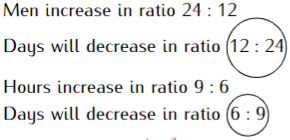
\includegraphics{Ratio_Ex2.png}
\[Days\, needed: \cancelto{\frac{1}{2}}{\frac{12}{24}}\times\cancelto{\frac{2}{3}}{\frac{6}{9}}\times12=4\]
\(\therefore\) The laborers would take \(4\) days

\end{tcolorbox}

\begin{tcolorbox}[enhanced jigsaw, leftrule=.75mm, opacityback=0, toprule=.15mm, bottomrule=.15mm, breakable, title=\textcolor{quarto-callout-note-color}{\faInfo}\hspace{0.5em}{Example 3}, opacitybacktitle=0.6, titlerule=0mm, colframe=quarto-callout-note-color-frame, rightrule=.15mm, coltitle=black, colback=white, bottomtitle=1mm, toptitle=1mm, left=2mm, colbacktitle=quarto-callout-note-color!10!white, arc=.35mm]

A blend of juice is made from mango and passion. The cost of four limes
of mango is \(Ksh.\, 180\) and two limes of passion is \(Ksh. \,160\).
In what ratio should the juice be mixed such that by selling the mixture
at \(Ksh.\, 90\) per lime, a profit of 20\% is realized? \hspace{5.5 cm}
\((3 mks)\)

\end{tcolorbox}

\begin{tcolorbox}[enhanced jigsaw, leftrule=.75mm, opacityback=0, toprule=.15mm, bottomrule=.15mm, breakable, title=\textcolor{quarto-callout-caution-color}{\faFire}\hspace{0.5em}{Solution}, opacitybacktitle=0.6, titlerule=0mm, colframe=quarto-callout-caution-color-frame, rightrule=.15mm, coltitle=black, colback=white, bottomtitle=1mm, toptitle=1mm, left=2mm, colbacktitle=quarto-callout-caution-color!10!white, arc=.35mm]

\begin{tabular}{|l|c|c|r|}
\hline
Juice&Mango&Passion&Blend\\
\hline
Ratio&1&n&$1+n$\\
\hline
cost  per litre&45&80&\,\\
\hline
Total cost&45&80n&45+80n\\
\hline
\end{tabular}

\[
\begin{split}
Buying \,price (B.P) \Rightarrow \frac{45+80n}{1+n}&=100\%\\
Selling \,Price (S.P) \Rightarrow 90&=120\%\\
B.P \Rightarrow \frac{90\times 10\cancel{0}}{12\cancel{0}}&=75\\
\frac{45+80n}{1+n}&=75\\
\end{split}
\]

\[
\begin{split}
45+80n&=75+75n \\5n&=30\\
\frac{\cancel{5}n}{\cancel5}&=\frac{\cancelto{6}{30}}{\cancel5}\\
\frac{n}{1}&=\frac{6}{1}\\
\Rightarrow \frac{1}{n}&=\frac{1}{6}\\
\therefore 1:n&=1:6
\end{split}
\]

\end{tcolorbox}

\begin{tcolorbox}[enhanced jigsaw, leftrule=.75mm, opacityback=0, toprule=.15mm, bottomrule=.15mm, breakable, title=\textcolor{quarto-callout-note-color}{\faInfo}\hspace{0.5em}{Example 4}, opacitybacktitle=0.6, titlerule=0mm, colframe=quarto-callout-note-color-frame, rightrule=.15mm, coltitle=black, colback=white, bottomtitle=1mm, toptitle=1mm, left=2mm, colbacktitle=quarto-callout-note-color!10!white, arc=.35mm]

A cold water tap can fill a bath in 15 minutes while a hot water tap can
fill it in 10 minutes. The drainage pipe can empty it in 8 minutes. The
cold water and hot water taps are opened for 2 minutes. After two
minutes all three taps are opened. Find the total time taken to fill the
bath. \hspace {14.8 cm} \((3 mks)\)

\end{tcolorbox}

\begin{tcolorbox}[enhanced jigsaw, leftrule=.75mm, opacityback=0, toprule=.15mm, bottomrule=.15mm, breakable, title=\textcolor{quarto-callout-caution-color}{\faFire}\hspace{0.5em}{Solution}, opacitybacktitle=0.6, titlerule=0mm, colframe=quarto-callout-caution-color-frame, rightrule=.15mm, coltitle=black, colback=white, bottomtitle=1mm, toptitle=1mm, left=2mm, colbacktitle=quarto-callout-caution-color!10!white, arc=.35mm]

\textbf{The 3 taps rate of filling the bath in 1 min:} \[
\begin{split}
Cold \,water\, tap &=\frac{1}{15}& \\
Hot\, water \,tap &=\frac{1}{10}& \\
Drainage \,tap &=\frac{1}{8}& \\
\textbf{Fraction\, by \,hot \.and\, cold \,tap\, in \,2 min:}\\
\left (\frac{1}{15}+\frac{1}{10}\right)*2&=\frac{1}{3}
\end{split}
\] \textbf{Fraction of water unfilled}:

\[\Rightarrow 1-\frac{1}{3}=\frac{2}{3}\]

\textbf{Fraction of water by 3 taps in 1 min:}
\[\frac{1}{15}+\frac{1}{10}-\frac{1}{8}=\frac{1}{24}\]

\textbf{Time to fill the remaining water:}
\[\frac{2}{3}\div \frac{1}{24}\Rightarrow \frac{2}{\cancel{3}} \times \cancel{24}^8=16 \]

\(\therefore\) Total time \(\Rightarrow 16+2=18\) min.

\end{tcolorbox}

\begin{tcolorbox}[enhanced jigsaw, leftrule=.75mm, opacityback=0, toprule=.15mm, bottomrule=.15mm, breakable, title=\textcolor{quarto-callout-note-color}{\faInfo}\hspace{0.5em}{Example 5}, opacitybacktitle=0.6, titlerule=0mm, colframe=quarto-callout-note-color-frame, rightrule=.15mm, coltitle=black, colback=white, bottomtitle=1mm, toptitle=1mm, left=2mm, colbacktitle=quarto-callout-note-color!10!white, arc=.35mm]

A plastic container manufacturer increased the radius of a cylindrical
can by 22.5\% but, decreased its height by 30\%. Calculate in two
decimal places the percentage increase in the volume of the can.
\hspace{15cm}\((3mks)\)

\end{tcolorbox}

\begin{tcolorbox}[enhanced jigsaw, leftrule=.75mm, opacityback=0, toprule=.15mm, bottomrule=.15mm, breakable, title=\textcolor{quarto-callout-caution-color}{\faFire}\hspace{0.5em}{Solution}, opacitybacktitle=0.6, titlerule=0mm, colframe=quarto-callout-caution-color-frame, rightrule=.15mm, coltitle=black, colback=white, bottomtitle=1mm, toptitle=1mm, left=2mm, colbacktitle=quarto-callout-caution-color!10!white, arc=.35mm]

\[
\begin{split}
Volume&=\pi r^2h\\Old\, volume &=\pi r^2h&\\
New \,radius&=1.225r\\New\, height&=0.7h\\
New \,volume&=\pi(1.225r)^2(0.7h)\\
&=1.225^2\times 0.7\times r^2\times h\\
& \approx 1.05044\pi r^2h
\end{split}
\]

\[
\begin{split}
Volume\, increase&=1.05044\pi r^2h-\pi r^2h\\
&=0.05044\pi r^2h\\
Percentage \,increase &=\frac{Increase}{Old \,volume}\times 100\\
&=\frac{0.05044\cancel{\pi r^2h}}{\cancel{\pi r^2h}}\times 100\\ 
&\approx5.044\% \\ 
\therefore \% \,increase&=5.04\%
\end{split}
\]

\end{tcolorbox}

\begin{tcolorbox}[enhanced jigsaw, leftrule=.75mm, opacityback=0, toprule=.15mm, bottomrule=.15mm, breakable, title=\textcolor{quarto-callout-note-color}{\faInfo}\hspace{0.5em}{Problems to Solve}, opacitybacktitle=0.6, titlerule=0mm, colframe=quarto-callout-note-color-frame, rightrule=.15mm, coltitle=black, colback=white, bottomtitle=1mm, toptitle=1mm, left=2mm, colbacktitle=quarto-callout-note-color!10!white, arc=.35mm]

\begin{enumerate}
\def\labelenumi{\arabic{enumi}.}
\item
  A photograph is reduced in the ratio \(2:7\) for a newspaper, and
  further reduced in the ratio \(5:7\) for an exercise book. Find the
  ratio of the newspaper size to textbook size. \hspace{2 cm} \((3mks)\)
\item
  Five plows working 8 hours daily complete a piece of work in 6 days.
  How long will it take 12 plows working 5 hours a day to complete the
  same work? \hspace{4.6 cm} \((2mks)\)
\item
  There are two grades of beans, grade A and grade B. Grade A costs
  \(Ksh. \,100\) per kg and grade B costs \(Ksh.\, 80\) per kg. In what
  ratio must the two grades be mixed in order to produce a blend worth
  \(Ksh.\, 95\) per kg? \hspace{10.6cm} \((3mks)\)
\item
  A tradesman blends 340kg of tea costing \(Ksh. \,80\) per kg with
  160kg of tea costing \(Ksh.\, 100\) per kg. At what price must he sell
  the mixture, to make a 25\% profit? \hspace{3.6cm} \((3mks)\)
\item
  Oil flows through a pipe whose cross-sectional radius is 7cm at a rate
  of 2m/min. Calculate how long it will take the pipe to fill a 28,000
  litres tank. \hspace{5.5cm} \((3 mks)\)
\item
  Nyamu and Gatungo working together can do a piece of work in 6 days.
  Gatungo working alone would take 10 days to complete the work. They
  start working together but, after 4 days Gatungo leaves and the
  remaining work is done by Nyamu. Find how long Nyamu takes to complete
  the remaining work. \hspace{11.5 cm} \((4mks)\)
\item
  Five constructors can build a 25-meter-long wall in 10 days. What
  length of wall can 10 constructors working at the same rate build in 8
  days? \hspace{5.8 cm} \((3mks)\)
\item
  A businesswoman bought 160 mangoes at \(Ksh. 50\) for every four
  mangoes. She sold some of them at \(Ksh. \,30\) for every three and
  the rest at \(Ksh.\, 30\) for every four. If she made a
  33\(\frac{1}{2}\)\% loss, calculate the number of mangoes sold at
  \(Ksh.\, 30\) for every four. \hspace{5 cm} \((3mks)\)
\item
  One hundred and twenty examiners each marking 90 papers per day are
  needed to mark an examination in 2 weeks. How many days would 180
  examiners each marking 35 papers per day take to mark the same
  examination? \hspace{8.2 cm} \((3mks)\)
\item
  A group of 15 soldiers set off with enough food to last 6 days. After
  6 soldiers evacuated. How many more days will the food last for the
  remaining soldiers? \hspace{4 cm} \((3 mks)\)
\item
  In the Moi University Christian Union choir, the ratio of male to
  female is \(2:3\). On one Sunday service, 10 male members were absent
  and six new female members joined the choir as guests for that day. If
  on this day the ratio of males to females was,\$ 1:3\$,, how many
  regular members does the choir have? \hspace{11.8 cm} \((3mks)\)
\item
  The ratio of men to women in Njega Boys High School B.O.G which
  consists of 45 members is \(7: 2\). Find the number of women required
  to join the existing members so that the ratio of men to women changes
  to \(5: 4\). \hspace{10.1cm} \((3mks)\)
\item
  A coffee trader mixes two brands of coffee, A and B to obtain 40kg of
  the mixture worth \(Ksh.\, 2,600\). If brand A is valued at
  \(Ksh.\, 70\) per kg and brand B is valued at \(Ksh.\, 55\) per kg.
  Calculate the ratio in its simplest form in which brands A and B are
  mixed. \hspace{3.7 cm} \((4mks)\)
\item
  Nyamu bought sorghum and millet at \(Ksh.\,65\) per kg and
  \(Ksh.\,40\) per kg respectively. He then mixed them and sold the
  mixture at \(Ksh.\,60\) per kg making a profit of 20\%. Determine the
  ratio of sorghum to millet in the mixture. \hspace{8.5 cm} \((3mks)\)
\item
  The ratio of a spherical balloon increases by 4\% as it rises up in
  the air. Find the percentage increase in its;

  a) Surface area. \hspace{11 cm} \((2mks)\)

  b) Volume \hspace{12 cm} \((2mks)\)
\item
  A dealer has two types of grades of tea, x and y. Grade x costs
  \(Ksh.\, 150\) per kg and grade y costs \(Ksh.\, 170\) per kg. If he
  mixes \(x\) and \(y\) in the ratio \(2:3\) to make a brand of tea
  which he sells at \(Ksh.\, 180\) per kg, calculate the percentage
  profit that he makes.\hspace{2.5cm} \((3 mks)\)
\item
  In what ratio will coffee grade A cost \(Ksh.\, 85\) per kg to be
  mixed with grade B costing \(Ksh.\,55\) per kg so that a profit of
  25\% is realized by selling the mixture at \(ksh.\,80\) per kg?
  \hspace{14.2cm} \((3mks)\)
\item
  A mixture contains two powders A and B with masses in the ration
  \(4: 10\). If the mixture costs \(Ksh.\, 650\) per kg and powder A
  costs \(Ksh. \,550\) per kg, find the cost of a kg of powder B.
  \hspace{14.1 cm} \((3 mks)\)
\item
  It would take 20 workers 12 days to spray a piece of land. If they
  work for 8 hours a day, how long will it take 24 workers if they work
  12 hours a day to three-quarters of the same land? \hspace{14.3cm}
  \((3mks)\)
\item
  A farmer has enough feed to last 35 pigs for 24 days. If he buys 5
  more pigs, how long will the feed last? \hspace{12.5 cm} \((3mks)\)
\item
  Mukami, a juice blender mixes two brands of Juice A and B to obtain
  90ml of the mixture worth \(Ksh.\, 165\) per litre. If brand A is
  valued at \(Ksh.\, 175\) per 1 litre bottle and brand B at
  \(Ksh.\, 150\) per 1-litre bottle, calculate the ratio in which the
  bands A and B are mixed.\hspace{3cm} \((2mks)\)
\item
  Twelve men can build 6 huts in 21 days. Find the number of men working
  at the same rate that will build 9 similar huts in 14 days.
  \hspace{8.5cm} \((3mks)\)
\item
  A rectangular dam with a surface area of 24 ares has a uniform depth
  of 5 m is to be drained for renovation. A pipe drains it at the rate
  of 250 litres per second. How long does it take to empty the dam?
  \hspace{12.7 cm} \((2mks)\)
\item
  Tap A can fill a tank in 12 minutes while tap B can fill the same tank
  in 15 minutes. Another tap C can empty the tank when full in 20
  minutes. Starting with an empty tank, the three taps are left open for
  4 minutes after which tap A is closed. How much longer does it take to
  fill the tank? \hspace{13.2 cm} \((3mks)\)
\item
  The radius of a cylindrical tin is increased by 20\% while its height
  is decreased by 10\%. If the capacity of the old tin is \(250\,cm^3\),
  find the capacity of the new tin. \hspace{4cm} \((3mks)\)
\item
  The radius of a cylindrical container is increased by 28\% while its
  height is reduced by 15\%. In 4 significant figures find the
  percentage increase in the volume of the juice in the
  container.\hspace{0cm} \((3mks)\)
\item
  Pipe X and Y can fill a tank in 15 minutes and 30 minutes
  respectively. Pipe Z can empty the full tank in 25 minutes. Starting
  with an empty tank, how long does it take to fill the tank if:

  a) All the three pipes are open? \hspace{8.6 cm} \((1mk)\)

  b) Pipe Y is closed after 10 minutes? \hspace{7.8 cm} \((3mks)\)
\item
  \(2,280 \,cm^3\), of milk was shared by three children, Josephine,
  Florence, and Moses in the ratio
  \(\frac{1}{4}:\frac{1}{2}:\frac{1}{5}\),, What volume did Moses get:
  \hspace{8.2 cm} \((2mks)\)
\item
  Sewage is flowing through a cylindrical pipe at the speed of
  \(0.95\,m/s\). If the pipe has an internal radius of 14cm, Calculate:

  a) The volume of sewage delivered by the pipe per second in \(cm^3\)
  (Take = \(\frac{22}{7}\)) \hspace{1 cm} \((2mks)\)

  b) The depth to which the pipe fills a rectangular tank of base
  dimensions \(6.5m \times 5.2m\) in one hour to the nearest 0.1 metres.
  \hspace{8.5 cm} \((3mks)\)

  c) The time is taken, to the nearest second for the pipe to fill a
  50,000-litre tank tub (initially empty) which has a hole at the base
  that drains the tub at the rate of 524 litres per minute.
  \hspace{13.5 cm} \((5mks)\)
\item
  Three potters; A, B, and C work together to make a certain number of
  pots. If Potter C was to work alone he would take 4\(\frac{4}{9}\),
  hours to complete the job. If all working together they will take 1hr
  40min to complete the job. They all started working together however,
  potter B left after the first 40 minutes, while Potter C left 20min
  later. Potter A took a further 1hr 46min. Calculate how long it would
  take if all the potters were made by:

  a) Potter A alone? \hspace{10.8 cm} \((6mks)\)

  b) Potter B alone? \hspace{10.8 cm} \((2mks)\)

  c) Potter A and C alone? \hspace{9.8 cm} \((2mks)\)
\item
  Boniface purchased 3 brands of coffee A, B, and C. The cost prices of
  the brands were \(Ksh.\, 50\), \(Ksh.\, 68\) and \(Ksh. \,75\) per
  kilogram respectively. He mixed the brands in the ratio of \(7:5:3\)
  respectively. After selling the mixture, he made a profit of 32\%.

  a) How much profit did he make per kilogram of the mixture?
  \hspace{4 cm} \((4mks)\)

  b) After one year, the cost price of each brand was increased by 15\%.

  i) For how much did he sell one kilogram of the mixture to make 20\%
  Profit.\hspace{1.3cm} \((3mks)\)

  ii) What would have been his percentage profit if he sold one kilogram
  of the mixture at \(Ksh. \,85.60\)? \hspace{10.6 cm} \((3mks)\)
\item
  A solution whose volume is 160 litres is made up of 75\% milk and the
  rest water. When x litres of milk is added the percentage of water
  drops to 20\%

  a) Find the value of \(x\) \hspace{10.4 cm} \((4mks)\)

  b) The new solution is diluted further by the addition of 120 litres
  of water. Calculate the percentage of milk in the resulting solution.
  \hspace{7.7 cm} \((2mks)\)

  c) A blend is made by mixing 10 litres of the solution in (b) above
  with 20 liters of the original solution. Calculate in the simplest
  form, the ratio of water to that of milk in the blend.
  \hspace{13.5 cm} \((4mks)\)
\item
  Four hundred and twenty litres of homogeneous paint is made by mixing
  three paints P, Q, and R. The ratio by volume of paint P to point Q is
  \(3: 4\) and paint Q to paint R is \(1: 2\). Paint P costs
  \(Ksh.\, 150\) per litre, paint Q \(Ksh. \,180\) per litre and paint R
  \(Ksh.\, 120.50\) per litre. Determine:

  a) The volume of each type of paint in the mixture. \hspace{5.9 cm}
  \((5mks)\)

  b) The amount of money spent in making one litre of the mixture.
  \hspace{3.5 cm} \((3mks)\)

  c) The percentage profit made by selling the mixture at \(Ksh.\, 205\)
  per litre. \hspace{1.7cm} \((2mks)\)
\item
  Olemapenzi's cows decreased by 16\% in 2014 to stand at 2100 cows at
  the beginning of 2015. The number of cows increased by 24\% in 2015
  and also increased by 20\% in 2016.

  a) Determine the number of cows Olemapenzi had at the beginning of:

  i) The year 2014 \hspace{10.4cm} \((2mks)\)

  ii) The year 2016 \hspace{10cm} \((2mks)\)

  iii) The year 2017 \hspace{10cm} \((2mks)\)

  b) Determine the percentage increase in Olemapenzi's cows between:

  i) 2014 and 2016 \hspace{10cm} \((2mks)\)

  ii) 2014 and 2017 \hspace{10cm} \((2mks)\)
\end{enumerate}

\end{tcolorbox}

\bookmarksetup{startatroot}

\hypertarget{chapter-ten-length-area-volume-and-capacity}{%
\chapter{Chapter Ten: Length, Area, Volume, and
Capacity}\label{chapter-ten-length-area-volume-and-capacity}}

\bookmarksetup{startatroot}

\hypertarget{length-area-volume-and-capacity}{%
\chapter*{Length, Area, Volume, and
Capacity}\label{length-area-volume-and-capacity}}
\addcontentsline{toc}{chapter}{Length, Area, Volume, and Capacity}

\markboth{Length, Area, Volume, and Capacity}{Length, Area, Volume, and
Capacity}

\textbf{Length}, is the distance between two points. Its SI Unit is the
meter (m). The perimeter of a rectangle and a square is given by the
formula: \[ Perimeter\, of \,a \,rectangle\,=\,2(length+width)\]

\[Perimeter \,of \,a \,square\,=\,4 \times length\]

The circumference of a circle is given by the formula:

\[
\begin{align*}
Circumference \,of\, a \,circle &=\pi D\\&=2\pi r
\end{align*} 
\] The length of an arc (l) of a circle subtended by an angle,
\(\theta\) , at the center of the circle is given by the formula:

\[ l=\frac{\theta}{360}\times 2\pi r\]

\textbf{Area}, is the amount of surface enclosed within the boundaries
of a plane shape. Its SI unit is a square meter (\(m^2\)).

\textbf{Area of a rectangle (A):}

\[A=length (l)\times width(w)=lw\]

\textbf{Area of square (A):}

\[A=length \times length= l^2\]

\textbf{Area of a triangle (A): }

\[A=\frac{1}{2} \times base \times height\]

\textbf{Area of a parallelogram (A):}

\[A=base \times height\] \textbf{Area of a rhombus (A):}

\[A=base \times height   \]

OR

\[A=\frac{1st\, diagonal \times 2nd \,diagonal}{2}\]

\textbf{Area of a trapezium  (A):}

\[
\begin{align*}
A&=\frac{1}{2} \times height\times (sum \,of \,the\, two \,parallel \,sides)\\
&=\frac{1}{2} \times h \times (a+b)
\end{align*}
\]

\textbf{Area of a circle (A):}

\[A=\pi r^2\]

\textbf{Area of a sector subtended by an angle \,$\theta $\,at the center of a circle:}

\[A=\frac{\theta}{360} \times\pi r^2\]

\centerline{\textbf{Surface area of solids (S.A)}}

\textbf{Surface area of a cuboid:}

\[
\begin{align*}
S.A&=2(length \times width)+2(width \times height)+2(length\times height)\\
&=2(lw)+2(wh)+2(lh)\\
&=2(lw+wh+lh)
\end{align*}
\]

\textbf{Surface area of a cylinder:} \[
\begin{align*}
S.A&=2\pi rh+2\pi r^2\\&=2\pi r(h+r)
\end{align*}
\]

\textbf{Surface area of a sphere:}

\[S.A=4\pi r^2\]

\textbf{Volume}, is the amount of space occupied by a matter. Its SI
unit is a cubic meter (\(m^3\)).

\textbf{Volume of a cuboid:} \[
\begin{align*}
v&=length \times width \times height\\&=lwh
\end{align*}
\]

\textbf{Volume of a cube:}

\[
\begin{align*}
v&=length \times length \times length \\
&=l^3 
\end{align*}
\]

\textbf{Volume of a cylinder:}

\[ v=\pi r^2 h\] \textbf{Volume of a sphere:}

\[ v=\frac{4}{3} \pi r^3\] \textbf{Volume of a prism:}

\[ 
\begin{align*}
v&=cross-sectional \,area \times length \\
&=\frac{1}{2}\times base\times height\times length\\
&=\frac{1}{2}\times bhl
\end{align*}
\]

\textbf{Capacity}, is the ability of the container to hold fluids. Its
SI unit is the litre (l).

\begin{tcolorbox}[enhanced jigsaw, leftrule=.75mm, opacityback=0, toprule=.15mm, bottomrule=.15mm, breakable, title=\textcolor{quarto-callout-note-color}{\faInfo}\hspace{0.5em}{Conversion of Units}, opacitybacktitle=0.6, titlerule=0mm, colframe=quarto-callout-note-color-frame, rightrule=.15mm, coltitle=black, colback=white, bottomtitle=1mm, toptitle=1mm, left=2mm, colbacktitle=quarto-callout-note-color!10!white, arc=.35mm]

\[ 
\begin{align*}
1 m &=100 cm \\ 
1 cm &= 10 mm\\ 
1000 cm^3 &= 1 \,litre =1 m^3\\
1 cm^3& = 1\, ml\\ 
10000 m^2 &= 1 \,hectare (ha)\\
100 m^2 &= 1 \,acre 
\end{align*}
\]

\end{tcolorbox}

\hypertarget{solved-examples-8}{%
\section{Solved Examples}\label{solved-examples-8}}

\begin{tcolorbox}[enhanced jigsaw, leftrule=.75mm, opacityback=0, toprule=.15mm, bottomrule=.15mm, breakable, title=\textcolor{quarto-callout-note-color}{\faInfo}\hspace{0.5em}{Example 1}, opacitybacktitle=0.6, titlerule=0mm, colframe=quarto-callout-note-color-frame, rightrule=.15mm, coltitle=black, colback=white, bottomtitle=1mm, toptitle=1mm, left=2mm, colbacktitle=quarto-callout-note-color!10!white, arc=.35mm]

An angle of 0.9 radians at the Centre of the circle subtends an arc of
length 28.8cm. Find in 4 significant figures(\(\pi radians=180^0\)):

\begin{enumerate}[(a)]
\item The radius of the circle              \hspace{10.4 cm}        $(3mks)$
\item The area of the sector enclosed by the arc and radii.     \hspace{5.5 cm} $(2mks)$
\end{enumerate}

\end{tcolorbox}

\begin{tcolorbox}[enhanced jigsaw, leftrule=.75mm, opacityback=0, toprule=.15mm, bottomrule=.15mm, breakable, title=\textcolor{quarto-callout-caution-color}{\faFire}\hspace{0.5em}{Solution}, opacitybacktitle=0.6, titlerule=0mm, colframe=quarto-callout-caution-color-frame, rightrule=.15mm, coltitle=black, colback=white, bottomtitle=1mm, toptitle=1mm, left=2mm, colbacktitle=quarto-callout-caution-color!10!white, arc=.35mm]

\textbf{The angle of the arc} \(=0.9 \pi radians\)

\textbf{Given that:} \(\pi\,rad=180^{0}\)

\textbf{The length of the arc (l) is given by:}

a)

\[ 
\begin{split}
\frac{\theta}{360}\times 2\pi r&=length\, of \,the \,arc \\
 28.8 cm &=\frac{162^{0}}{\cancel\pi}\times\frac{1}{\cancelto{180}{360}}\times \cancel2\cancel\pi r\\
\frac{162^{0}}{180^{0}}r &= 28.8 cm \\
r&= 28.8 cm \times \frac{180^{0}}{162^{0}}\\
\therefore r&=32
\end{split}
\]

b)

\[
\begin{split}
Area&=\frac{\theta}{360} \times\pi r^2 \\
&=\frac{162^{0}}{360^{0}\cancel\pi}\times\cancel\pi \times 32 \times 32\\
&=\frac{162^{0}}{360^{0}}\times 32 \times 32\\
&=460.8 cm^2
\end{split}
\]

\end{tcolorbox}

\begin{tcolorbox}[enhanced jigsaw, leftrule=.75mm, opacityback=0, toprule=.15mm, bottomrule=.15mm, breakable, title=\textcolor{quarto-callout-note-color}{\faInfo}\hspace{0.5em}{Example 2}, opacitybacktitle=0.6, titlerule=0mm, colframe=quarto-callout-note-color-frame, rightrule=.15mm, coltitle=black, colback=white, bottomtitle=1mm, toptitle=1mm, left=2mm, colbacktitle=quarto-callout-note-color!10!white, arc=.35mm]

A solid metal cylinder with a radius of 7cm and height of 5cm is melted
down and recast into a spherical ball. Calculate to 1 decimal place the
surface area of this ball.\hspace{5 cm} \((4mks)\)

\end{tcolorbox}

\begin{tcolorbox}[enhanced jigsaw, leftrule=.75mm, opacityback=0, toprule=.15mm, bottomrule=.15mm, breakable, title=\textcolor{quarto-callout-caution-color}{\faFire}\hspace{0.5em}{Solution}, opacitybacktitle=0.6, titlerule=0mm, colframe=quarto-callout-caution-color-frame, rightrule=.15mm, coltitle=black, colback=white, bottomtitle=1mm, toptitle=1mm, left=2mm, colbacktitle=quarto-callout-caution-color!10!white, arc=.35mm]

\textbf{Radius (R) of the cylinder:} \(R= 7cm\)

\textbf{Height (h) of the cylinder:} \(h= 5 cm\)

\textbf{Radius (r) of the sphere:} \(r=?\)

\textbf{Surface Area (S.A) of the Sphere:} \(S.A = 4\pi r^{2}\)

\[
\begin{split}
Volume\, of\, Cylinder &= volume\, of \,Sphere\\
\cancel\pi R^{2}h &= \frac{4}{3}\cancel\pi r^{3}\\
7^2\times5 &=\frac{4}{3}r^{3} \\
r^{3} &=7\times7\times5\times\frac{3}{4}\\
r &=\sqrt[3]{183.75}\\
\therefore r& \approx 5.685 cm\\
\end{split}
\]

\[
\begin{split}
S.A\,of\,the \,sphere& = 4\pi r^{2}\\
&=4\times\frac{22}{7}\times 5.685^{2}\\
&=406.299\\
&\approx 406.3 cm^{2}
\end{split}
\]

\end{tcolorbox}

\begin{tcolorbox}[enhanced jigsaw, leftrule=.75mm, opacityback=0, toprule=.15mm, bottomrule=.15mm, breakable, title=\textcolor{quarto-callout-note-color}{\faInfo}\hspace{0.5em}{Problems to Solve}, opacitybacktitle=0.6, titlerule=0mm, colframe=quarto-callout-note-color-frame, rightrule=.15mm, coltitle=black, colback=white, bottomtitle=1mm, toptitle=1mm, left=2mm, colbacktitle=quarto-callout-note-color!10!white, arc=.35mm]

\begin{enumerate}
\def\labelenumi{\arabic{enumi}.}
\item
  An arc of length `x' cm subtends an angle of, \((\frac{p}{\pi})^0\),at
  the center of the circle. Find an expression for the radius, r, of the
  circle in terms of x and p.~\hspace{6.2 cm} \((3mks)\)
\item
  Find the length of the minute hand of a wall clock if the tip of the
  minute hand traces a length of 6p cm between 11:25 am and 11:45 am
  (Give your answer in terms of \(\pi\)). \hspace{2 cm} \((3mks)\)
\item
  The diagonal of a rectangular flower garden is 20m. If the width of
  this garden is 12m, calculate its length and perimeter to 3
  significant figures. \hspace{6.7 cm} \((3mks)\)
\item
  The figure below shows a circle Centre O. Chord AB subtends \(30^0\)
  at the Centre. If the area of the minor segment is
  \(5\frac{16}{21} cm^2\), find the radius of the circle.(hint area of
  \(\triangle \,OAB=\frac{1}{2}r^2sin(\theta)\) \hspace{14.5cm}
  \((3mks)\)
\end{enumerate}

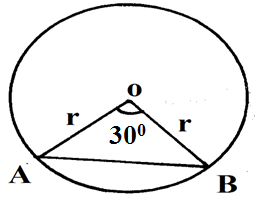
\includegraphics{circle.png}

\begin{enumerate}
\def\labelenumi{\arabic{enumi}.}
\setcounter{enumi}{4}
\item
  The curved surface area of a cylindrical container is \(2,112\,cm^2\).
  If the radius of the container is 21cm, calculate to one decimal place
  the capacity of the container in litres \hspace{2.1 cm} \((3mks)\)
\item
  The base of a triangle is 3cm longer than its height. Given that the
  area of the triangle is \(35cm^2\), determine the base of the
  triangle. \hspace{7.2 cm} \((3mks)\)
\item
  A carpenter constructed a closed wooden box with internal measurements
  1.8 m long, 0.8 m wide, and 0.6 m high. The wood used in constructing
  the box was 1.0cm thick and had a density of \(0.75g/cm^{3}\).
  Determine the:

  a) Volume in \(cm^3\) of the wood used in constructing the box.
  \hspace{4.2 cm} \((3mks)\)

  b) Mass of the box in kilograms correct to 4 significant figures.
  \hspace{3.6 cm} \((1mk)\)
\item
  A solid hemisphere of radius 7cm has the same volume as a cube. Find
  the length of the cube to 3 significant figures. \hspace{10.4 cm}
  \((3mks)\)
\item
  Mango juice in a factory is stored in a rectangular tank whose
  internal dimensions are 1.8m by 1.4m by 2.5m one day the tank was 80\%
  full of Mango juice. Calculate the volume of Mango juice in the tank
  in litres. \hspace{10 cm} \((3mks)\)
\item
  An open box has an external breadth of 12 cm, a height 10 cm, and a
  length of 15 cm. If the thickness of the material of the box is 1 cm,
  find the total surface area of the box. \hspace{3.7cm} \((5mks)\)
\item
  A triangular plot PQR is such that the length of the side PQ is
  two-thirds that of QR. The ratio of the lengths \(PQ: PR = 4:9\) and
  the angle at Q is obtuse. If the perimeter of the plot is 38m
  calculate the length of the 3 sides of \(\triangle PQR\)
  \hspace{7.5cm} \((4mks)\)
\item
  A metallic cuboid 10cm by 12cm by 15cm is melted. Half of it is used
  to make a cylinder of radius 4.2cm, the remaining is used to make a
  sphere. Determine in 4 significant figures using \(\pi= \frac{22}{7}\)

  a) The height and surface area of the cylinder to 2 decimal places.
  \hspace{3.2 cm} \((4mks)\)

  b) The radius and surface area of the sphere are correct to 3
  significant figures. \hspace{1.5 cm} \((4mks)\)

  c) The difference between the surface area of the sphere and the
  cylinder. \hspace{1.7cm} \((2mks)\)
\end{enumerate}

\end{tcolorbox}

\bookmarksetup{startatroot}

\hypertarget{chapter-eleven-mass-weight-and-density}{%
\chapter{Chapter Eleven: Mass, Weight and
Density}\label{chapter-eleven-mass-weight-and-density}}

\bookmarksetup{startatroot}

\hypertarget{mass-weight-and-density}{%
\chapter*{Mass, Weight and Density}\label{mass-weight-and-density}}
\addcontentsline{toc}{chapter}{Mass, Weight and Density}

\markboth{Mass, Weight and Density}{Mass, Weight and Density}

\textbf{Mass}, is the quantity of matter in an object? The Mass of an
object is constant everywhere. Its SI unit is Kilogram (K.g).

\textbf{Weight}, is the pull of the earth on an object. The weight of an
object varies from one place to another on the earth's surface. Its SI
unit is Newton (N). It is given by mass multiplied by the gravitational
force (g).

\(Weight (N) = mass (kg) \times gravity (N/kg).\)

\textbf{Density}, is mass per unit volume. Its SI unit is Kilogram per
Cubic meter (\(kgm^-3\))

\[Density= \frac{mass}{volume}\]
\[Density \,of\, mixture=\frac{mass \,of\, mixture}{volume\, of \,mixture} \]

\begin{tcolorbox}[enhanced jigsaw, leftrule=.75mm, opacityback=0, toprule=.15mm, bottomrule=.15mm, breakable, title=\textcolor{quarto-callout-note-color}{\faInfo}\hspace{0.5em}{Conversion of Units}, opacitybacktitle=0.6, titlerule=0mm, colframe=quarto-callout-note-color-frame, rightrule=.15mm, coltitle=black, colback=white, bottomtitle=1mm, toptitle=1mm, left=2mm, colbacktitle=quarto-callout-note-color!10!white, arc=.35mm]

\[
\begin{split}
1 \,tonne &= 1,000\, Kilograms\\
1 \,kilogram &= 1,000 \,grams\\
1g/cm^3& = 1,000 Kg/m^3
\end{split}
\]

\end{tcolorbox}

\hypertarget{solved-examples-9}{%
\section{Solved Examples}\label{solved-examples-9}}

\begin{tcolorbox}[enhanced jigsaw, leftrule=.75mm, opacityback=0, toprule=.15mm, bottomrule=.15mm, breakable, title=\textcolor{quarto-callout-note-color}{\faInfo}\hspace{0.5em}{Example 1}, opacitybacktitle=0.6, titlerule=0mm, colframe=quarto-callout-note-color-frame, rightrule=.15mm, coltitle=black, colback=white, bottomtitle=1mm, toptitle=1mm, left=2mm, colbacktitle=quarto-callout-note-color!10!white, arc=.35mm]

2.5 litres of water of density \(1g/cm^3\) is added to 4 litres of
alcohol of density \(0.8 g/cm^3\). Calculate in 3 significant figures,
the density of the mixture in its SI unit. \hspace{4.2 cm} (3mks)

\end{tcolorbox}

\begin{tcolorbox}[enhanced jigsaw, leftrule=.75mm, opacityback=0, toprule=.15mm, bottomrule=.15mm, breakable, title=\textcolor{quarto-callout-caution-color}{\faFire}\hspace{0.5em}{Solution}, opacitybacktitle=0.6, titlerule=0mm, colframe=quarto-callout-caution-color-frame, rightrule=.15mm, coltitle=black, colback=white, bottomtitle=1mm, toptitle=1mm, left=2mm, colbacktitle=quarto-callout-caution-color!10!white, arc=.35mm]

\[Density \,of \,Mixture (D.M)=\frac{Mass\, of\,mixture}{Volume\, of \,mixture}\]

\[
\begin{split}
Volume \,of \,water&=2,500 cm^3 \\
Mass \,of\, water&=(2,500 cm^3\times 1g/cm^3)\\
&=2,500g&\\
Volume\, of\, alcohol&=4,000 cm^3\\
Mass \,of \,alcohol&=(4,000 cm^3 \times 0.8g/cm^3)\\
&=3,200g
\end{split}
\]

\[
\begin{split}
Mass\, of\, Mixture&=(2,500g+3,200g)\\&=5,700g\\
Volume\, of \,mixture&=(2,500 cm^3+4,000 cm^3)\\&=6,500 cm^3\\
\therefore D.M&=\frac{5,7\cancel{0}\cancel{0}}{6,5\cancel{0}\cancel{0}}\\&=0.8769 g/cm^3\\
&=877 Kg/m^3
\end{split}
\]

\end{tcolorbox}

\begin{tcolorbox}[enhanced jigsaw, leftrule=.75mm, opacityback=0, toprule=.15mm, bottomrule=.15mm, breakable, title=\textcolor{quarto-callout-note-color}{\faInfo}\hspace{0.5em}{Example 2}, opacitybacktitle=0.6, titlerule=0mm, colframe=quarto-callout-note-color-frame, rightrule=.15mm, coltitle=black, colback=white, bottomtitle=1mm, toptitle=1mm, left=2mm, colbacktitle=quarto-callout-note-color!10!white, arc=.35mm]

wo coils of the same mass are made by winding zinc of different gauges
and lengths. The first coil is made by winding 648 m of wire with a
cross-sectional diameter of 5.4mm and the second coil is made by winding
450 m with different cross-sections. Find the cross-sectional radius of
the second coil. \((3mks)\)

\end{tcolorbox}

\begin{tcolorbox}[enhanced jigsaw, leftrule=.75mm, opacityback=0, toprule=.15mm, bottomrule=.15mm, breakable, title=\textcolor{quarto-callout-caution-color}{\faFire}\hspace{0.5em}{Solution}, opacitybacktitle=0.6, titlerule=0mm, colframe=quarto-callout-caution-color-frame, rightrule=.15mm, coltitle=black, colback=white, bottomtitle=1mm, toptitle=1mm, left=2mm, colbacktitle=quarto-callout-caution-color!10!white, arc=.35mm]

\textbf{Note:} Since mass is proportional to volume for the same
density, the volume of the first coil is equal to volume of the second
coil. \[
\begin{align*}
First\, coil \,volume:\\
\frac{22}{7}\times \left(\frac{5.4}{2}\right)^2\times 648,000&=14,846,605.71 \,mm^3\\
Second \,coil \,volume:\\
\frac{22}{7}\times r^2\times 450,000&=1,414,285.714r^2 \,mm^3\\
Second \,coil \,volume&=First\, coil \,volume\\
1,414,285.714r^2 \,mm^3&=14,846,605.71 \,mm^3\\
\frac{\cancel{1,414,285.714}r^2}
{\cancel{1,414,285.714}}&=\frac{\cancelto{10.4976}{14,846,605.71}}{\cancel{1,414,285.714}}\\r^2&=10.4976 \,mm^2\\
\therefore r&=3.24\, mm
\end{align*}
\]

\end{tcolorbox}

\begin{tcolorbox}[enhanced jigsaw, leftrule=.75mm, opacityback=0, toprule=.15mm, bottomrule=.15mm, breakable, title=\textcolor{quarto-callout-note-color}{\faInfo}\hspace{0.5em}{Example 3}, opacitybacktitle=0.6, titlerule=0mm, colframe=quarto-callout-note-color-frame, rightrule=.15mm, coltitle=black, colback=white, bottomtitle=1mm, toptitle=1mm, left=2mm, colbacktitle=quarto-callout-note-color!10!white, arc=.35mm]

The external measurements of a closed metal box are 1.6 m long, 0.7 m
wide, and 0.4 m high. The metal used in making box is 1.0 cm thick and
has a density of 0.85 g/cm3. If the box contains 40 packets of 12
similar tools each and each tool has a mass of 115 g, calculate:

\begin{enumerate}[(a)]
\item The volume of metal used in making the box.   \hspace{7cm}        $(4mks)$
\item The mass of the empty box in Kilograms to 3 significant figures.      \hspace{4cm}    $(3mks)$
\item The total mass of the box in kilograms to 3 significant figures.      \hspace{4.5cm}      $(3mks)$
\end{enumerate}

\end{tcolorbox}

\begin{tcolorbox}[enhanced jigsaw, leftrule=.75mm, opacityback=0, toprule=.15mm, bottomrule=.15mm, breakable, title=\textcolor{quarto-callout-caution-color}{\faFire}\hspace{0.5em}{Solution}, opacitybacktitle=0.6, titlerule=0mm, colframe=quarto-callout-caution-color-frame, rightrule=.15mm, coltitle=black, colback=white, bottomtitle=1mm, toptitle=1mm, left=2mm, colbacktitle=quarto-callout-caution-color!10!white, arc=.35mm]

\begin{enumerate}[(a)]
\item 
\begin{align*}
\textbf{Volume of the Cuboid (v):} \\
v&=Length\times Width\times Height\\
\textbf{External\, Measurement: }\\
Length&=160 cm\\
Width&=70 cm\\
Height&=40 cm\\
\textbf{Internal\, Measurement:} \\
thickness&=1 cm\\
Length&=158 cm\\
\end{align*}

\begin{align*}
Width&=68 cm\\
Height&=38 cm\\ \textbf{External\, volume:} \\
160\times 70\times 40&=448,000\,cm^3\\ \textbf{Internal\, Volume:}\\
158\times 68 \times 38&=408,272\,cm^3\\
448,000\,cm^3-408,272\,cm^3&=39,728\,cm^3\\ \therefore Volume\, of\,the\,metal&=39,728 \,cm^3
\end{align*}

\item 
\begin{align*}
Mass&=density\times volume\\
&=0.85 g/cm^3\times 39,728 cm^3\\ 
&=33,768.8g\\
\frac{33,768.8}{1000}&=33.7688 \,Kg\\
\therefore Mass \,of\, the\, empty \,box&=33.8\,Kg
\end{align*}

\item 
\begin{align*}
Mass\: of \:tools:\\
12\times 40 \times 115&=55,200\, g\\
 \frac{55,200}{1000}&=55.2 \, Kg\\
\therefore The\: total\: Mass&=55.2+33.8\\
&=89.0 \,Kg
\end{align*}
\end{enumerate}

\end{tcolorbox}

\begin{tcolorbox}[enhanced jigsaw, leftrule=.75mm, opacityback=0, toprule=.15mm, bottomrule=.15mm, breakable, title=\textcolor{quarto-callout-note-color}{\faInfo}\hspace{0.5em}{Problems to Solve}, opacitybacktitle=0.6, titlerule=0mm, colframe=quarto-callout-note-color-frame, rightrule=.15mm, coltitle=black, colback=white, bottomtitle=1mm, toptitle=1mm, left=2mm, colbacktitle=quarto-callout-note-color!10!white, arc=.35mm]

\begin{enumerate}
\def\labelenumi{\arabic{enumi}.}
\item
  A solid block in the shape of a cylinder has a height of 14cm and
  weighs 26kg. If it is made of material of density \(0.45g/cm^3\), find
  the radius of the cylinder to four significant figures. Take
  \(\pi=\frac{22}{7}\) \hspace{13.7 cm} \((3mks)\)
\item
  \(2000 cm\^3\) of a mixture consists of 2.5 kg of substance x and 7.5
  kg of substance y. find the density of mixture in \(g/cm^3\)
  \hspace{11 cm} \((3mks)\)
\item
  An artisan has 63kg of metal of density \(7g/cm^3\). He intends to use
  it to make a rectangular pipe with external dimensions 12cm by 15cm
  and internal dimensions 10cm by 12 cm. Calculate the length of the
  pipe in metres. \hspace{9.8 cm} \((3mks)\)
\item
  A solid metal cuboid 2.1m long, 0.8m wide, and 0.75m high of material
  of density \(0.75g/cm^3\). Calculate its mass in kilograms.
  \hspace{8.8 cm} \((2mks)\)
\item
  A metal R is an alloy of two metals X and Y. Metal X has a mass of 70g
  and a density of \(16000kg/m^3\). Metal Y has a mass of 42g and a
  density of \(4000 kg/m^3\). In 4 significant figures, calculate the
  density of the metal R in its SI unit. \hspace{6cm} \((4mks)\)
\item
  Two coils of the same mass are made by winding aluminum wire of
  different gauges and lengths. If the first coil is made by winding 540
  m of the wire with diameter 1.96 mm cross-sectional diameter and the
  second coil is made by winding a certain length of the wire with a
  cross-sectional diameter of 2.94 mm, find the length of the second
  coil wire. \hspace{4.3cm} \((3mks)\)
\item
  The external measurements of a wooden box are 1.2 m long, 65 cm wide,
  and 40 cm high. The wood used in making the box is 2 cm thick and has
  a density of \(950 Kg/m^3\). Given that the box contains 30 packets of
  tools and each packet holds a dozen tools each weighing 125 g,
  calculate:

  a) The volume of wood used in making the box. \hspace{6cm} \((4mks)\)

  b) The mass of the empty box in kilograms to four significant figures.
  \hspace{3cm}\((3mks)\)

  c) The total mass of the box in kilograms to 3 significant figures.
  \hspace{3.8cm}\((3mks)\)
\end{enumerate}

\end{tcolorbox}

\bookmarksetup{startatroot}

\hypertarget{chapter-twelve-time}{%
\chapter{Chapter Twelve: Time}\label{chapter-twelve-time}}

\bookmarksetup{startatroot}

\hypertarget{time}{%
\chapter*{Time}\label{time}}
\addcontentsline{toc}{chapter}{Time}

\markboth{Time}{Time}

\textbf{Time} can be given in either a 12-hour clock system or a 24-hour
system. In a 12-hour system, time is counted from midnight (12:00
midnight). The time is written as am from midnight to midday and pm from
midday to midnight. In the 24-hour clock system, time is expressed in
hours and counted from midnight to midnight.

To convert a 12-hour clock system to a 24-hour system, add 12 to a pm
time. To convert a 24-hour time to a 12-hour time, subtract 12 if it's
13 or more, then add the right suffix (am if the original value is less
than 13, or pm if the original value is 13 or more).

\begin{tcolorbox}[enhanced jigsaw, leftrule=.75mm, opacityback=0, toprule=.15mm, bottomrule=.15mm, breakable, title=\textcolor{quarto-callout-note-color}{\faInfo}\hspace{0.5em}{Problems to Solve}, opacitybacktitle=0.6, titlerule=0mm, colframe=quarto-callout-note-color-frame, rightrule=.15mm, coltitle=black, colback=white, bottomtitle=1mm, toptitle=1mm, left=2mm, colbacktitle=quarto-callout-note-color!10!white, arc=.35mm]

\begin{enumerate}
\def\labelenumi{\arabic{enumi}.}
\item
  A car left town A for town B at 1000h and had a puncture after
  traveling for 2 h 30 min fixing a new tyre took 36 minutes. The car
  then traveled for another 1 hour 45 min before reaching town B. At
  what time did it arrive? \hspace{9.7 cm} \((3mks)\)
\item
  An airplane left Nairobi at 2045h and arrived in London at 0320h. It
  stayed for \(1\frac{1}{2}\) hours for rest and refreshment of
  passengers and crew. It then headed for Washington D.C and took
  \(9 \frac{1}{4}\) hours.
\end{enumerate}

a) How long did the journey from Nairobi to London take in hours and
minutes? \hspace{0.5 cm} \((2mks)\)

b) At what time did it arrive in Washington D.C.? \hspace{5.6 cm}
\((2mks)\)

\begin{enumerate}
\def\labelenumi{\arabic{enumi}.}
\setcounter{enumi}{2}
\item
  A watch that loses a half-minute every hour was set to read the
  correct time at 0445h on Monday. Determine the time, in the 12-hour
  system, the watch will show on the following Friday at 1845h.
  \hspace{13 cm} \((3mks)\)
\item
  The average lap time for 3 athletes in a long-distance race is 36
  seconds, 40 seconds, and 48 seconds respectively. If they all start
  the race at the same time, find the number of times the slowest runner
  will have been overlapped by the fastest at the time they all cross
  the starting point together again. \hspace{10.7 cm} \((3mks)\)
\item
  The travel timetable below shows the departure and arrival time for a
  bus plying between two towns M and R, 450 kilometers apart.
\end{enumerate}

\begin{center}
    \begin{tabular}{l|c|r} 
      \textbf{TOWN} & \textbf{ARRIVAL} & \textbf{DEPARTURE}\\
      \hline
      M & &0830h \\
      N &       1000h   &       1020h \\
P       &   1310h       &   1340h \\
Q       &   1510h       &   1520h \\
R       &   1600h&         \\

\end{tabular}
\end{center}

\begin{enumerate}
\def\labelenumi{\arabic{enumi}.}
\setcounter{enumi}{5}
\tightlist
\item
  Calculate the average speed for the whole journey. \hspace{7 cm}
  \((3mks)\)
\end{enumerate}

\end{tcolorbox}

\bookmarksetup{startatroot}

\hypertarget{chapter-15-linear-equations}{%
\chapter{Chapter 15: Linear
Equations}\label{chapter-15-linear-equations}}

\bookmarksetup{startatroot}

\hypertarget{linear-equations}{%
\chapter*{Linear Equations}\label{linear-equations}}
\addcontentsline{toc}{chapter}{Linear Equations}

\markboth{Linear Equations}{Linear Equations}

Linear equations are equations of straight lines involving one or two
unknown variables. A system of two linear equations forms simultaneous
equations.

There are three methods used to solve simultaneous equations:

\begin{itemize}
\tightlist
\item
  \textbf{Elimination method}
\item
  \textbf{Substitution method}
\item
  \textbf{Graphical method}
\end{itemize}

\hypertarget{solved-examples-10}{%
\section{Solved examples}\label{solved-examples-10}}

\hypertarget{substitution-method}{%
\subsection{Substitution method}\label{substitution-method}}

\begin{tcolorbox}[enhanced jigsaw, leftrule=.75mm, opacityback=0, toprule=.15mm, bottomrule=.15mm, breakable, title=\textcolor{quarto-callout-note-color}{\faInfo}\hspace{0.5em}{Example 1}, opacitybacktitle=0.6, titlerule=0mm, colframe=quarto-callout-note-color-frame, rightrule=.15mm, coltitle=black, colback=white, bottomtitle=1mm, toptitle=1mm, left=2mm, colbacktitle=quarto-callout-note-color!10!white, arc=.35mm]

\[
\begin{align*}
2x-3y&=-13... \hspace{3.3cm} (i)\\
y&=2x+7 ...   \hspace{2.6cm} (ii)
\end{align*}
\]

\end{tcolorbox}

\begin{tcolorbox}[enhanced jigsaw, leftrule=.75mm, opacityback=0, toprule=.15mm, bottomrule=.15mm, breakable, title=\textcolor{quarto-callout-caution-color}{\faFire}\hspace{0.5em}{Solution}, opacitybacktitle=0.6, titlerule=0mm, colframe=quarto-callout-caution-color-frame, rightrule=.15mm, coltitle=black, colback=white, bottomtitle=1mm, toptitle=1mm, left=2mm, colbacktitle=quarto-callout-caution-color!10!white, arc=.35mm]

\[
  Substituting\, equation \,(ii) \,into \,(i);
 \begin{align*}
 2x-3(2x+7)&=-13\\
 2x-6x-21&=-13\\
-4x &= -13 + 21\\
 \frac{\cancel{-4}x}{\cancel{-4}}& = \frac{\cancelto{-2}{8}}{\cancel{-4}} \\x&=-2\\  \end{align*}
 \]

\[  
  \begin{align*}
 but,\, y&=2x+7\\
 Solve\, for\, y:\\
 y&=2(-2)+7\\
 &=3\\ \therefore Solution \,set&=(-2,3)
 \end{align*}
\]

\end{tcolorbox}

\begin{tcolorbox}[enhanced jigsaw, leftrule=.75mm, opacityback=0, toprule=.15mm, bottomrule=.15mm, breakable, title=\textcolor{quarto-callout-note-color}{\faInfo}\hspace{0.5em}{Example 2}, opacitybacktitle=0.6, titlerule=0mm, colframe=quarto-callout-note-color-frame, rightrule=.15mm, coltitle=black, colback=white, bottomtitle=1mm, toptitle=1mm, left=2mm, colbacktitle=quarto-callout-note-color!10!white, arc=.35mm]

\[
\begin{align*}
7x + 15y &= 22...\hspace{2cm} (i)\\
8x + 17y &= 25...\hspace{2cm} (ii)\\
\end{align*}
\]

\end{tcolorbox}

\begin{tcolorbox}[enhanced jigsaw, leftrule=.75mm, opacityback=0, toprule=.15mm, bottomrule=.15mm, breakable, title=\textcolor{quarto-callout-caution-color}{\faFire}\hspace{0.5em}{Solution}, opacitybacktitle=0.6, titlerule=0mm, colframe=quarto-callout-caution-color-frame, rightrule=.15mm, coltitle=black, colback=white, bottomtitle=1mm, toptitle=1mm, left=2mm, colbacktitle=quarto-callout-caution-color!10!white, arc=.35mm]

\[
\begin{align*}
Solving\, for\, x\, in \,(i);\\
x&=\frac{22-15y}{7}\\
substituting \,x=\frac{22-15y}{7} \,in \,(ii)\\
8\left(\frac{22-15y}{7}\right)+17y&=25\\
Multiplying \,both\, side\, by \,7;\\
176-120y+119y&=175\\
\cancel{-}y&=\cancel{-}1\\
y&=1\\ then \, , \,x&=\frac{22-15(1)}{7}\\
&x=1\\
\therefore Solution \,set&=(1,1)
\end{align*}
\]

\end{tcolorbox}

\hypertarget{elimination-method}{%
\subsection{Elimination method}\label{elimination-method}}

\begin{tcolorbox}[enhanced jigsaw, leftrule=.75mm, opacityback=0, toprule=.15mm, bottomrule=.15mm, breakable, title=\textcolor{quarto-callout-note-color}{\faInfo}\hspace{0.5em}{Example 3}, opacitybacktitle=0.6, titlerule=0mm, colframe=quarto-callout-note-color-frame, rightrule=.15mm, coltitle=black, colback=white, bottomtitle=1mm, toptitle=1mm, left=2mm, colbacktitle=quarto-callout-note-color!10!white, arc=.35mm]

\[
\begin{align*}
3x-7y&=13... \hspace{2cm} (i)\\
6x - 5y& = 8...  \hspace{2.1cm} (ii)
\end{align*}
\]

\end{tcolorbox}

\begin{tcolorbox}[enhanced jigsaw, leftrule=.75mm, opacityback=0, toprule=.15mm, bottomrule=.15mm, breakable, title=\textcolor{quarto-callout-caution-color}{\faFire}\hspace{0.5em}{Solution}, opacitybacktitle=0.6, titlerule=0mm, colframe=quarto-callout-caution-color-frame, rightrule=.15mm, coltitle=black, colback=white, bottomtitle=1mm, toptitle=1mm, left=2mm, colbacktitle=quarto-callout-caution-color!10!white, arc=.35mm]

To eliminate x multiply equation (i) by 2 and (ii) by 1 and then
subtract (ii) from (i);

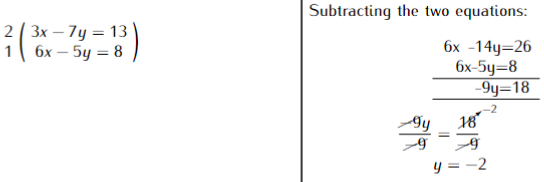
\includegraphics{Li_eq_Ex3.png}

Plugging y=-2 in (i) or (ii) to determine the value of x;

\[
\begin{align*}
3x-7(-2)&=13\\
3x+14&=13\\3x&=-1\\
\frac{\cancel{3}x}{\cancel{3}}&=-\frac{1}{3}\\
x&=\frac{-1}{3}\\ Solution\, set&=(-\frac{1}{3},-2)
\end{align*}
\]

\end{tcolorbox}

\begin{tcolorbox}[enhanced jigsaw, leftrule=.75mm, opacityback=0, toprule=.15mm, bottomrule=.15mm, breakable, title=\textcolor{quarto-callout-note-color}{\faInfo}\hspace{0.5em}{Example 4 \hspace{11.5 cm} \((4mks)\)}, opacitybacktitle=0.6, titlerule=0mm, colframe=quarto-callout-note-color-frame, rightrule=.15mm, coltitle=black, colback=white, bottomtitle=1mm, toptitle=1mm, left=2mm, colbacktitle=quarto-callout-note-color!10!white, arc=.35mm]

\[\frac{x+y}{6}-\frac{x+y}{4}=-\frac{1}{4} \]
\[\frac{x-y}{5} + \frac{x-y}{6}=1\frac{1}{10}\]

\end{tcolorbox}

\begin{tcolorbox}[enhanced jigsaw, leftrule=.75mm, opacityback=0, toprule=.15mm, bottomrule=.15mm, breakable, title=\textcolor{quarto-callout-caution-color}{\faFire}\hspace{0.5em}{Solution}, opacitybacktitle=0.6, titlerule=0mm, colframe=quarto-callout-caution-color-frame, rightrule=.15mm, coltitle=black, colback=white, bottomtitle=1mm, toptitle=1mm, left=2mm, colbacktitle=quarto-callout-caution-color!10!white, arc=.35mm]

Simplifying the two equations;

Multiply the 1st equation by 12;

\[\left(\frac{x+y}{6}-\frac{x+y}{4}=\frac{-1}{4}\right)12\]
\[2x+2y-3x-3y=-3\] \[-x-y=-3 \,\ldots \ldots\ldots(i)\]

Multiply the 2nd equation by 30;

\[\left(\frac{x-y}{5}+\frac{x-y}{6}=\frac{11}{10}\right)30\]
\[6x-6y+5x-5y=33\]

\[11x-11y=33 \, \ldots\ldots\ldots (ii)\]

Multiply equation (i) by 11 and add to equation (ii) to eliminate x;

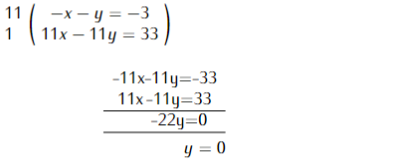
\includegraphics{Li_eq_Ex4.png}

Plugging \(y= 0\) in (i) or (ii) to determine the value of x;

\[
\begin{align*}
-x-y(0)&=-3\\
-x&=-3\\x&=3\\
\therefore Solution \,set&=(3,0)
\end{align*}
\]

\end{tcolorbox}

\begin{tcolorbox}[enhanced jigsaw, leftrule=.75mm, opacityback=0, toprule=.15mm, bottomrule=.15mm, breakable, title=\textcolor{quarto-callout-note-color}{\faInfo}\hspace{0.5em}{Problems to Solve}, opacitybacktitle=0.6, titlerule=0mm, colframe=quarto-callout-note-color-frame, rightrule=.15mm, coltitle=black, colback=white, bottomtitle=1mm, toptitle=1mm, left=2mm, colbacktitle=quarto-callout-note-color!10!white, arc=.35mm]

\begin{enumerate}
\def\labelenumi{\arabic{enumi}.}
\tightlist
\item
  Solve the following equations \hspace{9.5 cm} \((4mks)\)
\end{enumerate}

\[
\begin{split}
\frac{3y-2x}{15}+\frac{2x+1}{3}&=2\\
\frac{2x-3y}{15}-\frac{1-x}{3}&=1
\end{split}
\]

\begin{enumerate}
\def\labelenumi{\arabic{enumi}.}
\setcounter{enumi}{1}
\item
  Solve the simultaneous equations. \hspace{8.7 cm} \((3mks)\) \[
  \begin{align*}
  2x+3y &= 4\\
  x + 4y &= 7
  \end{align*}
  \]
\item
  Solve the simultaneous equations: \hspace{8.5 cm} \((3mks)\)
\end{enumerate}

\[
\begin{align*}
2x -y+ 2 &= 0 \\
-3y + x &= -6 
\end{align*}
\]

\begin{enumerate}
\def\labelenumi{\arabic{enumi}.}
\setcounter{enumi}{3}
\item
  Mercy a student at Mucagara mixed Secondary bought 5 pens and 3
  exercise books from Magunas supermarket at Ksh. 135, at the same time
  Murugi her class mate also bought 4 pens and 5 exercise books and
  spent Ksh. 25 more than Mercy. Find the cost of each pen and exercise
  book. \hspace{13.2 cm} \((4mks)\)
\item
  In July, Kiama donated \(\frac{1}{6}\)th of his salary to a children's
  home while Joshua donated \(\frac{1}{5}\)th of his salary to the same
  children's home. Their total donation for July was \(Ksh.\, 14,820\).
  In August, Kiama donated \(\frac{1}{8}\)th of his salary to the
  children's home while Joshua donated \(\frac{1}{12}\)th of his salary
  to the children's home. Their total donation for August was
  \(Ksh.\, 8,675\). Calculate Kiama's monthly salary. \hspace{13.1 cm}
  \((4mks)\)
\item
  Three spoons and four plates cost \(Ksh. \,87\). Two spoons and five
  plates cost \(Ksh.\, 93\). Find the cost of one spoon and one plate.
  \hspace{9cm} \((4mks)\)
\item
  Mwendia bought 8 pairs of trousers and six socks at \(Ksh.\, 4,160\).
  Had he bought twice as many socks and half as many trousers, he would
  have saved \(Ksh.\, 100\). Find the cost of each item. \hspace{14.3cm}
  \((3mks)\)
\item
  Esther bought 144 mangoes at \(Ksh.\, 100\) for every six mangoes. She
  sold some of them at \(Ksh.\, 72\) for every three and the rest at
  \(Ksh.\, 60\) for every two. If she made a 45\% profit, calculate the
  number of mangoes sold at \(Ksh.\, 72\) for every three.
  \hspace{7.1cm} \((3mks)\)
\item
  Four men took their cows to the market. John had two more cows than
  Enoch. Alex had as many cows as John, whereas Jeff had 10 cows less
  than the sum of both John and Alex.

  a) Write a simplified expression with one variable, representing the
  total number of cows. \hspace{13.6cm} \((1mk)\)

  b) Three butchers bought all the cows and shared them equally. If each
  butcher got 17 cows, how many did Jeff sell to the butchers
  \hspace{7.5 cm} \((3mks)\)
\item
  Wanjiru bought three cups and four plates for Ksh. 324. Moraa bought
  five cups and Anyango bought two plates of the same type as those
  bought by Wanjiru. Moraa paid \(Ksh.\, 228\) more than Anyango. Find
  the price of each cup and spoon. \hspace{5.4cm} \((3mks)\)
\item
  Daniel and Sokoro bought the same types of pens and blades from the
  same shop. Daniel bought 2 pens and 3 blades for \(Ksh.\, 78\). Sokoro
  bought 3 pens and 4 blades and spent \(Ksh.\, 36\) more than Daniel.
  Calculate the cost of each item \hspace{6cm} \((3mks)\)
\item
  Karani bought 4 pencils and 6 blades for \(Ksh.\, 66\) and Kanuni
  bought 2 pencils and 5 blades for \(Ksh.\, 51\).

  a) Find the price of each item.\hspace{9cm} \((3mks)\)

  b) Naomi spent Ksh. 228 to buy the same type of pencils and blades. If
  the number of blades she bought was 4 more than the number of pencils,
  find the number of pencils bought. \hspace{13.5cm} \((3mks)\)
\item
  A retailer bought 50 plates and 30 spoons from a wholesaler P for
  \(Ksh.\, 4260\). Had she bought 15 plates less and half spoons more,
  she would have paid \(Ksh. \,990\) less. Had the retailer bought from
  wholesaler Q, she would have paid 50\% more for a plate and 25\% less
  for a spoon. How much would she have lost if she had bought the 50
  plates and the 30 spoons from wholesaler Q.? \hspace{14.2 cm}
  \((10mks)\)
\end{enumerate}

\end{tcolorbox}

\bookmarksetup{startatroot}

\hypertarget{chapter-fourteen-commercial-arithmetic}{%
\chapter{Chapter Fourteen: Commercial
Arithmetic}\label{chapter-fourteen-commercial-arithmetic}}

\bookmarksetup{startatroot}

\hypertarget{chapter-fifteen-co-ordinates-and-graphs}{%
\chapter{Chapter Fifteen: Co-Ordinates and
Graphs}\label{chapter-fifteen-co-ordinates-and-graphs}}

\bookmarksetup{startatroot}

\hypertarget{chapter-sixteen-angles-and-plane-figures}{%
\chapter{Chapter Sixteen: Angles and Plane
Figures}\label{chapter-sixteen-angles-and-plane-figures}}

\bookmarksetup{startatroot}

\hypertarget{chapter-seventeen-geometrical-constructions}{%
\chapter{Chapter Seventeen: Geometrical
Constructions}\label{chapter-seventeen-geometrical-constructions}}

\bookmarksetup{startatroot}

\hypertarget{geometrical-constructions}{%
\chapter*{Geometrical Constructions}\label{geometrical-constructions}}
\addcontentsline{toc}{chapter}{Geometrical Constructions}

\markboth{Geometrical Constructions}{Geometrical Constructions}

\bookmarksetup{startatroot}

\hypertarget{chapter-eighteen-scale-drawing}{%
\chapter{Chapter Eighteen: Scale
Drawing}\label{chapter-eighteen-scale-drawing}}

I love this

\hypertarget{bearing-and-distance-angles-of-elevation-and-depression}{%
\section{Bearing and Distance, Angles of Elevation and
Depression}\label{bearing-and-distance-angles-of-elevation-and-depression}}

\bookmarksetup{startatroot}

\hypertarget{section-two}{%
\chapter*{SECTION TWO}\label{section-two}}
\addcontentsline{toc}{chapter}{SECTION TWO}

\markboth{SECTION TWO}{SECTION TWO}

\bookmarksetup{startatroot}

\hypertarget{model-samples-papers}{%
\chapter*{Model Samples Papers}\label{model-samples-papers}}
\addcontentsline{toc}{chapter}{Model Samples Papers}

\markboth{Model Samples Papers}{Model Samples Papers}

\hypertarget{model-sample-paper-1}{%
\section*{model Sample Paper 1}\label{model-sample-paper-1}}
\addcontentsline{toc}{section}{model Sample Paper 1}

\markright{model Sample Paper 1}

\hypertarget{model-sample-paper-2}{%
\section*{model Sample Paper 2}\label{model-sample-paper-2}}
\addcontentsline{toc}{section}{model Sample Paper 2}

\markright{model Sample Paper 2}

\hypertarget{model-sample-paper-3}{%
\section*{model Sample Paper 3}\label{model-sample-paper-3}}
\addcontentsline{toc}{section}{model Sample Paper 3}

\markright{model Sample Paper 3}

\hypertarget{model-sample-paper-4}{%
\section*{model Sample Paper 4}\label{model-sample-paper-4}}
\addcontentsline{toc}{section}{model Sample Paper 4}

\markright{model Sample Paper 4}

\hypertarget{model-sample-paper-5}{%
\section*{model Sample Paper 5}\label{model-sample-paper-5}}
\addcontentsline{toc}{section}{model Sample Paper 5}

\markright{model Sample Paper 5}

\hypertarget{model-sample-paper-6}{%
\section*{model Sample Paper 6}\label{model-sample-paper-6}}
\addcontentsline{toc}{section}{model Sample Paper 6}

\markright{model Sample Paper 6}

\hypertarget{model-sample-paper-7}{%
\section*{model Sample Paper 7}\label{model-sample-paper-7}}
\addcontentsline{toc}{section}{model Sample Paper 7}

\markright{model Sample Paper 7}

\hypertarget{model-sample-paper-8}{%
\section*{model Sample Paper 8}\label{model-sample-paper-8}}
\addcontentsline{toc}{section}{model Sample Paper 8}

\markright{model Sample Paper 8}

\hypertarget{model-sample-paper-9}{%
\section*{model Sample Paper 9}\label{model-sample-paper-9}}
\addcontentsline{toc}{section}{model Sample Paper 9}

\markright{model Sample Paper 9}

\hypertarget{model-sample-paper-10}{%
\section*{model Sample Paper 10}\label{model-sample-paper-10}}
\addcontentsline{toc}{section}{model Sample Paper 10}

\markright{model Sample Paper 10}

\bookmarksetup{startatroot}

\hypertarget{section-three}{%
\chapter*{SECTION THREE}\label{section-three}}
\addcontentsline{toc}{chapter}{SECTION THREE}

\markboth{SECTION THREE}{SECTION THREE}

\bookmarksetup{startatroot}

\hypertarget{answers-to-problems-to-solve}{%
\chapter*{Answers to Problems to
Solve}\label{answers-to-problems-to-solve}}
\addcontentsline{toc}{chapter}{Answers to Problems to Solve}

\markboth{Answers to Problems to Solve}{Answers to Problems to Solve}

\hypertarget{chapter-1-natural-numbers-1}{%
\section*{chapter 1: Natural
Numbers}\label{chapter-1-natural-numbers-1}}
\addcontentsline{toc}{section}{chapter 1: Natural Numbers}

\markright{chapter 1: Natural Numbers}

\hypertarget{rounding-off-1}{%
\subsection*{Rounding Off}\label{rounding-off-1}}
\addcontentsline{toc}{subsection}{Rounding Off}

\hypertarget{operations-1}{%
\subsection*{Operations}\label{operations-1}}
\addcontentsline{toc}{subsection}{Operations}

\hypertarget{chapter-2-factors-1}{%
\section*{Chapter 2: Factors}\label{chapter-2-factors-1}}
\addcontentsline{toc}{section}{Chapter 2: Factors}

\markright{Chapter 2: Factors}

\hypertarget{chapter-3-divisibility-test}{%
\section*{Chapter 3: Divisibility
Test}\label{chapter-3-divisibility-test}}
\addcontentsline{toc}{section}{Chapter 3: Divisibility Test}

\markright{Chapter 3: Divisibility Test}

\hypertarget{chapter-4-g.c.d-and-l.c.m-1}{%
\section*{Chapter 4: G.C.D and
L.C.M}\label{chapter-4-g.c.d-and-l.c.m-1}}
\addcontentsline{toc}{section}{Chapter 4: G.C.D and L.C.M}

\markright{Chapter 4: G.C.D and L.C.M}

\hypertarget{chapter-5-integers-1}{%
\section*{Chapter 5: Integers}\label{chapter-5-integers-1}}
\addcontentsline{toc}{section}{Chapter 5: Integers}

\markright{Chapter 5: Integers}

\hypertarget{chapter-6-fractions-1}{%
\section*{Chapter 6: Fractions}\label{chapter-6-fractions-1}}
\addcontentsline{toc}{section}{Chapter 6: Fractions}

\markright{Chapter 6: Fractions}

\hypertarget{chapter-7-decimals-squares-and-square-roots}{%
\section*{Chapter 7: Decimals, Squares, and Square
Roots}\label{chapter-7-decimals-squares-and-square-roots}}
\addcontentsline{toc}{section}{Chapter 7: Decimals, Squares, and Square
Roots}

\markright{Chapter 7: Decimals, Squares, and Square Roots}

\hypertarget{chapter-8-algebraic-expression}{%
\section*{Chapter 8: Algebraic
Expression}\label{chapter-8-algebraic-expression}}
\addcontentsline{toc}{section}{Chapter 8: Algebraic Expression}

\markright{Chapter 8: Algebraic Expression}

\hypertarget{chapter-9-rate-ratio-proportion-and-percentage}{%
\section*{Chapter 9: Rate, Ratio, Proportion, and
Percentage}\label{chapter-9-rate-ratio-proportion-and-percentage}}
\addcontentsline{toc}{section}{Chapter 9: Rate, Ratio, Proportion, and
Percentage}

\markright{Chapter 9: Rate, Ratio, Proportion, and Percentage}

\hypertarget{chapter-10-length-area-volume-and-capacity}{%
\section*{Chapter 10: Length, Area, Volume, and
Capacity}\label{chapter-10-length-area-volume-and-capacity}}
\addcontentsline{toc}{section}{Chapter 10: Length, Area, Volume, and
Capacity}

\markright{Chapter 10: Length, Area, Volume, and Capacity}

\hypertarget{chapter-11-mass-weight-and-density}{%
\section*{Chapter 11: Mass, Weight, and
Density}\label{chapter-11-mass-weight-and-density}}
\addcontentsline{toc}{section}{Chapter 11: Mass, Weight, and Density}

\markright{Chapter 11: Mass, Weight, and Density}

\hypertarget{chapter-12-time}{%
\section*{Chapter 12: Time}\label{chapter-12-time}}
\addcontentsline{toc}{section}{Chapter 12: Time}

\markright{Chapter 12: Time}

\hypertarget{chapter-13-linear-equatins}{%
\section*{Chapter 13: Linear
Equatins}\label{chapter-13-linear-equatins}}
\addcontentsline{toc}{section}{Chapter 13: Linear Equatins}

\markright{Chapter 13: Linear Equatins}

\hypertarget{chapter-14-commercial-arithmetic}{%
\section*{Chapter 14: Commercial
Arithmetic}\label{chapter-14-commercial-arithmetic}}
\addcontentsline{toc}{section}{Chapter 14: Commercial Arithmetic}

\markright{Chapter 14: Commercial Arithmetic}

\hypertarget{chapter-15-co-ordinates-and-graphs}{%
\section*{Chapter 15: Co-Ordinates and
Graphs}\label{chapter-15-co-ordinates-and-graphs}}
\addcontentsline{toc}{section}{Chapter 15: Co-Ordinates and Graphs}

\markright{Chapter 15: Co-Ordinates and Graphs}

\hypertarget{chapter-16-angles-and-plane-figures}{%
\section*{Chapter 16: Angles and Plane
Figures}\label{chapter-16-angles-and-plane-figures}}
\addcontentsline{toc}{section}{Chapter 16: Angles and Plane Figures}

\markright{Chapter 16: Angles and Plane Figures}

\hypertarget{chapter-17-geometrical-constructions}{%
\section*{Chapter 17: Geometrical
Constructions}\label{chapter-17-geometrical-constructions}}
\addcontentsline{toc}{section}{Chapter 17: Geometrical Constructions}

\markright{Chapter 17: Geometrical Constructions}

\hypertarget{chapter-18-scale-drawing}{%
\section*{Chapter 18: Scale Drawing}\label{chapter-18-scale-drawing}}
\addcontentsline{toc}{section}{Chapter 18: Scale Drawing}

\markright{Chapter 18: Scale Drawing}

\bookmarksetup{startatroot}

\hypertarget{section-four}{%
\chapter*{SECTION FOUR}\label{section-four}}
\addcontentsline{toc}{chapter}{SECTION FOUR}

\markboth{SECTION FOUR}{SECTION FOUR}

\bookmarksetup{startatroot}

\hypertarget{answers-to-model-sample-papers}{%
\chapter*{Answers to Model Sample
Papers}\label{answers-to-model-sample-papers}}
\addcontentsline{toc}{chapter}{Answers to Model Sample Papers}

\markboth{Answers to Model Sample Papers}{Answers to Model Sample
Papers}

\hypertarget{model-sample-paper-1-1}{%
\section*{model Sample Paper 1}\label{model-sample-paper-1-1}}
\addcontentsline{toc}{section}{model Sample Paper 1}

\markright{model Sample Paper 1}

\hypertarget{model-sample-paper-2-1}{%
\section*{model Sample Paper 2}\label{model-sample-paper-2-1}}
\addcontentsline{toc}{section}{model Sample Paper 2}

\markright{model Sample Paper 2}

\hypertarget{model-sample-paper-3-1}{%
\section*{model Sample Paper 3}\label{model-sample-paper-3-1}}
\addcontentsline{toc}{section}{model Sample Paper 3}

\markright{model Sample Paper 3}

\hypertarget{model-sample-paper-4-1}{%
\section*{model Sample Paper 4}\label{model-sample-paper-4-1}}
\addcontentsline{toc}{section}{model Sample Paper 4}

\markright{model Sample Paper 4}

\hypertarget{model-sample-paper-5-1}{%
\section*{model Sample Paper 5}\label{model-sample-paper-5-1}}
\addcontentsline{toc}{section}{model Sample Paper 5}

\markright{model Sample Paper 5}

\hypertarget{model-sample-paper-6-1}{%
\section*{model Sample Paper 6}\label{model-sample-paper-6-1}}
\addcontentsline{toc}{section}{model Sample Paper 6}

\markright{model Sample Paper 6}

\hypertarget{model-sample-paper-7-1}{%
\section*{model Sample Paper 7}\label{model-sample-paper-7-1}}
\addcontentsline{toc}{section}{model Sample Paper 7}

\markright{model Sample Paper 7}

\hypertarget{model-sample-paper-8-1}{%
\section*{model Sample Paper 8}\label{model-sample-paper-8-1}}
\addcontentsline{toc}{section}{model Sample Paper 8}

\markright{model Sample Paper 8}

\hypertarget{model-sample-paper-9-1}{%
\section*{model Sample Paper 9}\label{model-sample-paper-9-1}}
\addcontentsline{toc}{section}{model Sample Paper 9}

\markright{model Sample Paper 9}

\hypertarget{model-sample-paper-10-1}{%
\section*{model Sample Paper 10}\label{model-sample-paper-10-1}}
\addcontentsline{toc}{section}{model Sample Paper 10}

\markright{model Sample Paper 10}



\end{document}
